\documentclass[UTF8, a4paper, 12pt]{ctexart}

% --- 核心宏包 ---
\usepackage{geometry}
\geometry{a4paper, margin=25.4mm} % 常用 1 英寸边距
\usepackage{amsmath, amssymb}
\usepackage{amsfonts}
\usepackage{xcolor} % 用于设置蓝色字体

% --- 全局排版设置 ---
\setlength{\parindent}{0pt} % 全局取消首行缩进
\setlength{\parskip}{0.5em}  % 设置段落间距,增加美观度

%---提示框---
\usepackage[most]{tcolorbox}
\tcbuselibrary{breakable}

%---画图---
% ===============================
% TikZ 绘图
% ===============================
\usepackage{tikz}
\usetikzlibrary{
  arrows.meta,
  calc,
  math,
  shadings,
  decorations.pathreplacing
} 
\usetikzlibrary{shapes, backgrounds}
\usepackage{pgfplots}
\pgfplotsset{compat=1.18}
\pgfmathdeclarefunction{gauss}{1}{%
  \pgfmathparse{1/sqrt(2*pi)*exp(-#1^2/2)}%
}
\usepgfplotslibrary{fillbetween} % 用于填充阴影
\usetikzlibrary{arrows.meta, shadings, shadows, fadings}
\pgfplotsset{compat=1.18}

% 定义一个柔和的渐变效果
\tikzfading[name=fade out, inner color=transparent!0, outer color=transparent!100]

\begin{document}


\begin{center}
\large{\textbf{BDIC2005J Probability and Statistics 2019-2020}}
\end{center}
\textbf{Question 1:} \\
\textbf{Vacancy (Each blank 3 marks)}

1. There are two events $A$ and $B$. $P(A)+P(B)=0.7$, $P(AB)=0.3$.  

Then, $P(A \cup B)=\underline{0.4}$, \quad $P(A\bar{B}) + P(\bar{A}B)=\underline{0.1}.$

{\color{blue}
\textbf{Solution:}

Given
\[
P(A)+P(B)=0.7, \qquad P(AB)=0.3.
\]

We have
\[
P(A\cup B)=P(A)+P(B)-P(AB)=0.7-0.3=0.4.
\]

We known that
\[
P(A\overline{B})=P(A)-P(AB), \qquad
P(\overline{A}B)=P(B)-P(AB).
\]

Hence,
\[
P(A\bar{B})+P(\bar{A}B)
= P(A)+P(B)-2P(AB)
= 0.7 - 2\times 0.3
= 0.1.
\]
}

\begin{tcolorbox}[
        enhanced,
        colback=blue!5,
        colframe=blue!50!black,
        width=\textwidth,
        arc=2mm, 
        title={解题方法:画图解决},
        breakable
]

\textbf{1. 几何方法:利用韦恩图分析该问题}
\begin{center}
\begin{tikzpicture}[fill opacity=0.5, scale=0.9]
    % 增大半径至 2.2cm,保持圆心距 1.6cm 以确保交集足够大
    \def\circleA{(0,0) circle (2.2cm)}
    \def\circleB{(1.6,0) circle (2.2cm)}

    % 1. 绘制 A 独有的区域 (左月牙) - 浅蓝色
    \begin{scope}
        \clip \circleA;
        \fill[blue!40] \circleA;
        \fill[white, opacity=1] \circleB;
    \end{scope}

    % 2. 绘制 B 独有的区域 (右月牙) - 浅橙色
    \begin{scope}
        \clip \circleB;
        \fill[orange!40] \circleB;
        \fill[white, opacity=1] \circleA;
    \end{scope}

    % 3. 绘制交集区域 (中间) - 浅绿色
    \begin{scope}
        \clip \circleA;
        \fill[green!30] \circleB;
    \end{scope}

    % 绘制圆的轮廓线
    \draw[thick] \circleA;
    \draw[thick] \circleB;
    
    % 标签位置:圆的正上方
    \node at (-0.5, 2.5) [opacity=1, font=\bfseries] {事件 $A$};
    \node at (2.1, 2.5) [opacity=1, font=\bfseries] {事件 $B$};
    
    % 内部区域标注,确保文字在较大圆内不拥挤
    \node at (0.8, 0) [opacity=1, font=\small] {$P(AB)=0.3$};
    \node at (-1.4, 0) [opacity=1, font=\small] {$P(A\bar{B})$};
    \node at (3.0, 0) [opacity=1, font=\small] {$P(\bar{A}B)$};
\end{tikzpicture}
\end{center}

\vspace{0.5em}
\textbf{2. 事件与韦恩图的对应关系解释}
\begin{itemize}
    \item \textbf{并集 $P(A \cup B)$}:对应图中所有的颜色区域。公式 $P(A)+P(B)-P(AB)$ 的意思是:$A$ 圆加 $B$ 圆时,中间的重叠部分被算了两次,所以要减去一次。
    \item $P(A\bar{B}) + P(\bar{A}B)$:对应图中 $A$ 独有和 $B$ 独有的部分(左右两个月牙)。公式 $P(A)+P(B)-2P(AB)$ 的意思是:从两个圆的总面积中把中间重叠的部分完全扣除。
\end{itemize}

\vspace{0.5em}
\textbf{3. 易错点}
\begin{itemize}
    \item 题目给出的条件是 $P(A)+P(B)$ 的“整体和”,不需要分别求出 $P(A)$ 或 $P(B)$ 的具体数值。
    \item 要区分“恰有一个发生”与“至少一个发生”的区别。
\end{itemize}

\end{tcolorbox}

2. Suppose the random variable $X$ follows the Poisson distribution with the parameter $\lambda=1$, $P(X=2)=\underline{\dfrac{e^{-1}}{2}}$ \quad ,
$E(X^2)=\underline{2}$.

{\color{blue}
\textbf{Solution:}

If $X\sim \text{Poisson}(\lambda=1)$.

Then
\[
P(X=k)=\frac{\lambda^k e^{-\lambda}}{k!}.
\]

Thus,
\[
P(X=2)=\frac{1^2 e^{-1}}{2!}=\frac{e^{-1}}{2}.
\]

For a Poisson random variable,
\[
E(X)=\lambda, \qquad \mathrm{Var}(X)=\lambda.
\]

Using
\[
E(X^2)=\mathrm{Var}(X)+[E(X)]^2,
\]

We obtain
\[
E(X^2)=1+1^2=2.
\]
}

\begin{tcolorbox}[
        enhanced,
        colback=green!2,
        colframe=green!40!black,
        width=\textwidth,
        arc=2mm, 
        title={要点:泊松分布},
        breakable
]

\textbf{1. 概率分布图示 (当 $\lambda=1$ 时)}

\begin{center}
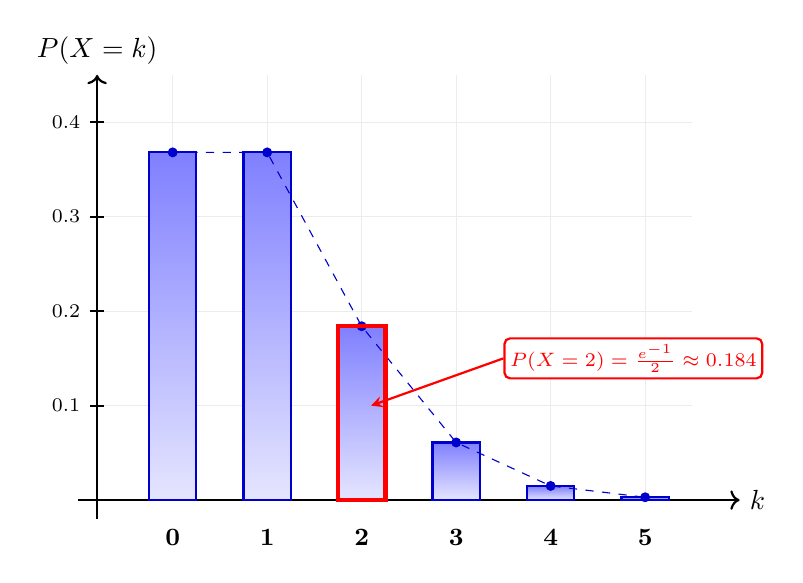
\begin{tikzpicture}[scale=1.2]
    % 1. 绘制网格背景 (向左延伸以覆盖y轴)
    \draw[very thin, gray!15] (-0.8,0) grid (5.5, 4.5);
    
    % 2. 绘制轴线 (y轴设在 x=-0.8 的位置,离 k=0 远一些)
    \draw[->, thick] (-1.0,0) -- (6,0) node[right] {$k$};
    \draw[->, thick] (-0.8,-0.2) -- (-0.8,4.5) node[above] {$P(X=k)$};
    
    % 3. 绘制纵轴刻度与数值 (对应概率 0.1, 0.2, 0.3, 0.4)
    \foreach \y/\ytext in {1/0.1, 2/0.2, 3/0.3, 4/0.4}
        \draw[shift={(-0.8,\y)}, thick] (2pt,0pt) -- (-2pt,0pt) node[left, font=\scriptsize] {\ytext};

    % 4. 绘制柱状图 - 使用蓝色渐变
    % 数据: P(0)=0.368, P(1)=0.368, P(2)=0.184, P(3)=0.061, P(4)=0.015
    \foreach \k/\p in {0/3.68, 1/3.68, 2/1.84, 3/0.61, 4/0.15, 5/0.03} {
        \draw[top color=blue!50, bottom color=blue!10, draw=blue!80!black, thick] 
            (\k-0.25,0) rectangle (\k+0.25, \p);
        \node at (\k, -0.4) [font=\small\bfseries] {\k};
    }
    
    % 5. 绘制趋势虚线 (Envelope curve)
    \draw[dashed, blue!80!black, thin] (0,3.68) -- (1,3.68) -- (2,1.84) -- (3,0.61) -- (4,0.15) -- (5,0.03);
    \foreach \k/\p in {0/3.68, 1/3.68, 2/1.84, 3/0.61, 4/0.15, 5/0.03}
        \fill[blue!80!black] (\k,\p) circle (1.5pt);

    % 6. 重点标注 P(X=2)
    \draw[red, ultra thick] (1.75,0) rectangle (2.25, 1.84); % 红色边框高亮
    \draw[red, <-, >=stealth, thick] (2.1, 1.0) -- (3.5, 1.5) 
        node[right, fill=white, draw=red, rounded corners=2pt, inner sep=2pt, font=\scriptsize, opacity=1] 
        {$P(X=2) = \frac{e^{-1}}{2} \approx 0.184$};
\end{tikzpicture}
\end{center}

\vspace{0.5em}

\textbf{2. 泊松分布的特征}
\begin{itemize}
    \item \textbf{形状}:当 $\lambda=1$ 时,泊松分布在 $k=0$ 和 $k=1$ 处取得最大概率(均为 $e^{-1}$)。随着 $k$ 的增大,概率呈阶乘级速度衰减。
    \item \textbf{二阶矩的意义}:$E(X^2)$ 指的是把随机变量平方之后再取期望。
    \item \textbf{二阶矩与方差的关系}: \\
    随机变量 $X$ 的方差定义为:$\operatorname{Var}(X)=E\big[(X-E(X))^2\big]$。 \\
    对平方项展开,有$(X-E(X))^2 = X^2 - 2XE(X) + [E(X)]^2$。 \\
    因此,$\operatorname{Var}(X) =E(X^2 - 2XE(X) + [E(X)]^2)$。 \\
    利用期望的线性性质,展开得到$\operatorname{Var}(X)=E(X^2) - 2E(X)E(X) + [E(X)]^2$。\\
    化简可得$\operatorname{Var}(X)=E(X^2)-[E(X)]^2$。 \\
    等价地,也可以写为$E(X^2)=\operatorname{Var}(X)+[E(X)]^2$。\\
    即,二阶矩 = 方差 + 均值的平方
\end{itemize}

\vspace{0.5em}
\textbf{3. 技巧点}
\begin{itemize}
    \item 泊松分布的“期望等于方差”:$E(X) = \text{Var}(X) = \lambda$。
    \item 记住: $E(X^2) = \lambda^2 + \lambda$ 。
\end{itemize}

\end{tcolorbox}

3. Suppose the random variables $X$ and $Y$ are mutually independent, $X \sim N(3,3^2)$, $Y \sim N(1,2^2)$, \quad $Z=X-2Y$, $Z \sim \underline{N(1,25)}$, \quad $P(-4<Z<6)=\underline{0.6826}$. \\
$(\Phi(1)=0.8413)$

{\color{blue}
\textbf{Solution:}

Since $X$ and $Y$ are independent and normally distributed, $Z$ is also normally distributed.
\[
E(Z)=E(X)-2E(Y)=3-2\times 1=1,
\]
\[
\mathrm{Var}(Z)=\mathrm{Var}(X)+4\mathrm{Var}(Y)=3^2+4\times 2^2=9+16=25.
\]

Therefore,
\[
Z\sim N(1,25).
\]

Standardize $Z$:
\[
P(-4<Z<6)
= P\left(\frac{-4-1}{5}<\frac{Z-1}{5}<\frac{6-1}{5}\right)
= P(-1<Z_0<1),
\]

where $Z_0\sim N(0,1)$.

Using $\Phi(1)=0.8413$,
\[
P(-1<Z_0<1)=2\Phi(1)-1=2\times 0.8413-1=0.6826.
\]
}

\begin{tcolorbox}[
    enhanced,
    colback=blue!5,
    colframe=blue!60!black,
    arc=2mm,
    title={提示:正态分布的线性性质与标准化},
    fonttitle=\bfseries,
    breakable
]

\textbf{1. 正态分布的线性性质}

若随机变量 $X$ 与 $Y$ 相互独立,且
$X\sim N(\mu_X,\sigma_X^2)$, $Y\sim N(\mu_Y,\sigma_Y^2)$,则线性组合仍然服从正态分布:
\[
aX+bY \sim N\big(a\mu_X+b\mu_Y,\; a^2\sigma_X^2+b^2\sigma_Y^2\big).
\]

\bigskip

\textbf{2. 关键点}

\begin{itemize}
    \item \textbf{均值计算:} $E(X-2Y) = E(X) - 2E(Y) = 3 - 2(1) = 1$。
    \item \textbf{方差计算:} $\text{Var}(X-2Y) = \text{Var}(X) + (-2)^2\text{Var}(Y)$。\\
    注意:中间是减号,但方差贡献是系数平方相加,即 $3^2 + 4 \times 2^2 = 25$。
\end{itemize}

\bigskip

\textbf{3. 标准化}

本题计算 $P(-4 < Z < 6)$ 等价于计算标准正态分布 $Z_0$ 在 $\pm 1$ 个标准差之间的面积:
\[
P\left( \frac{-4-1}{5} < Z_0 < \frac{6-1}{5} \right) = P(-1 < Z_0 < 1)
\]

\bigskip

\textbf{4. 标准正态分布图示}
\begin{center}
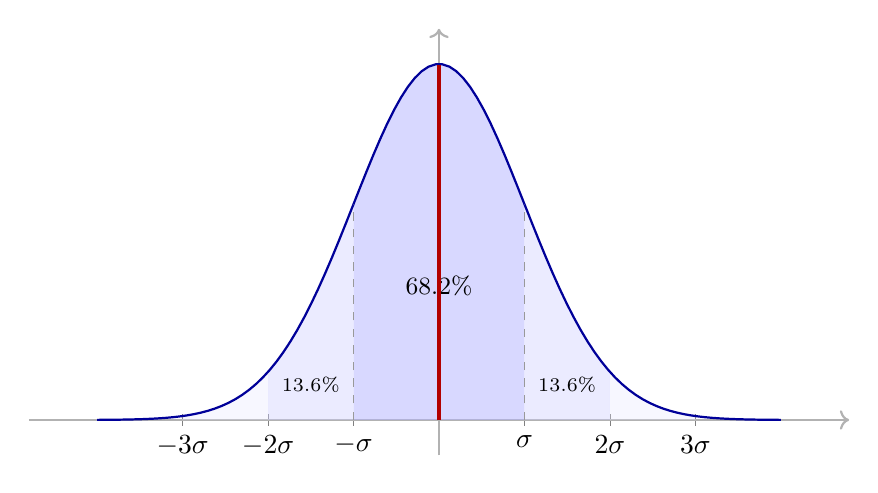
\begin{tikzpicture}
\begin{axis}[
    width=12cm, height=7cm,
    axis lines=middle,
    enlargelimits=true,
    samples=100,
    domain=-4:4,
    ytick=\empty,
    xtick={-3,-2,-1,0,1,2,3},
    xticklabels={$-3\sigma$, $-2\sigma$, $-\sigma$, $\mu$, $\sigma$, $2\sigma$, $3\sigma$},
    every axis x label/.style={at={(current axis.right of origin)},anchor=north west},
    axis line style={->, thick, gray!60},
]

% 1. 定义正态分布函数
\addplot [name path=curve, thick, blue!60!black, domain=-4:4] 
    {1/(sqrt(2*pi))*exp(-0.5*x^2)};

% 2. 建立基准线(用于填充阴影)
\path [name path=axis] (axis cs:-4,0) -- (axis cs:4,0);

% 3. 填充不同标准差范围的阴影(质感核心)
% 填充 68% 区域 (1 sigma)
\addplot [fill=blue!30, opacity=0.5] fill between [
    of=curve and axis, soft clip={domain=-1:1}
];
% 填充 95% 区域 (2 sigma)
\addplot [fill=blue!20, opacity=0.4] fill between [
    of=curve and axis, soft clip={domain=-2:-1}
];
\addplot [fill=blue!20, opacity=0.4] fill between [
    of=curve and axis, soft clip={domain=1:2}
];
% 填充 99.7% 区域 (3 sigma)
\addplot [fill=blue!10, opacity=0.3] fill between [
    of=curve and axis, soft clip={domain=-3:-2}
];
\addplot [fill=blue!10, opacity=0.3] fill between [
    of=curve and axis, soft clip={domain=2:3}
];

% 4. 添加标注百分比
\node at (axis cs:0, 0.15) {\small $68.2\%$};
\node at (axis cs:1.5, 0.04) {\scriptsize $13.6\%$};
\node at (axis cs:-1.5, 0.04) {\scriptsize $13.6\%$};

% 5. 装饰性的垂直虚线
\draw [dashed, gray!80] (axis cs:1,0) -- (axis cs:1,0.242);
\draw [dashed, gray!80] (axis cs:-1,0) -- (axis cs:-1,0.242);
\draw [very thick, red!70!black] (axis cs:0,0) -- (axis cs:0,0.398);

\end{axis}
\end{tikzpicture}
\end{center}

\end{tcolorbox}


\textbf{Question 2: (14 marks)}

A company $X$ has three factories $F_1$, $F_2$ and $F_3$, all of which produce similar automotive parts. Suppose that $F_1$, $F_2$ and $F_3$ produce $20\%$, $45\%$ and $35\%$ of the total production, respectively. On the average, $2\%$ of the parts produced by $F_1$ is unqualified. For $F_2$ and $F_3$, the corresponding unqualified percent are $5\%$ and $1\%$, respectively.

1. Find the probability that an automotive part produced by the company $X$ is unqualified;

2. If one product was selected randomly and found to be unqualified, what is the probability that it was made by $F3$.



{\color{blue}
\textbf{Solution:}

1. Let $U$ denote the event that a product is unqualified.

Define $P(F_{i})$ the probability that the product was produced in $F_{i}$, then
\[
P(F_1)=0.20, \quad P(F_2)=0.45, \quad P(F_3)=0.35.
\]

The corresponding unqualified rates are
\[
P(U|F_1)=0.02, \quad P(U|F_2)=0.05, \quad P(U|F_3)=0.01.
\]

By the law of total probability,
\[
\begin{aligned}
P(U)
&= P(F_1)P(U|F_1) + P(F_2)P(U|F_2) + P(F_3)P(U|F_3) \\
&= 0.20\times 0.02 + 0.45\times 0.05 + 0.35\times 0.01 \\
&= 0.004 + 0.0225 + 0.0035 \\
&= 0.03.
\end{aligned}
\]

2. By Bayes' theorem,
\[
P(F_3|U)=\frac{P(F_3)P(U|F_3)}{P(U)}
=\frac{0.35\times 0.01}{0.03}
=\frac{0.0035}{0.03}
=\frac{7}{60}.
\]
}

\begin{tcolorbox}[
        enhanced,
        colback=white,
        colframe=blue!50!black,
        width=\textwidth,
        arc=2mm, auto outer arc,
        title={提示:全概率公式与贝叶斯定理},
        fonttitle=\bfseries,
        breakable
]

\textbf{一、 事件}
\begin{itemize}
    \item \textbf{完备事件组}:本题中工厂 $F_1, F_2, F_3$ 构成了样本空间的一个划分(即产品只能由这三家工厂之一生产,且三者概率之和为 1)。
    \item \textbf{条件概率}:题目中给出的“某工厂生产的不合格率”即为条件概率 $P(U|F_i)$,而非联合概率。
\end{itemize}

\textbf{二、 概率树}
\smallskip

% --- TikZ 概率树图示 ---
\begin{center}
\begin{tikzpicture}[
    level 1/.style={level distance=2.5cm, sibling distance=2.5cm},
    level 2/.style={level distance=2.5cm, sibling distance=1.2cm},
    edge from parent/.style={draw, ->, >=latex, thick},
    every node/.style={font=\small}
]

% 根节点
\node {产品来源}
    child {node {$F_1$} 
        child {node {$U$ (不合格)} edge from parent node[left, pos=0.6] {\scriptsize $0.02$}}
        child {node {$\bar{U}$} edge from parent node[right, pos=0.6] {\scriptsize $0.98$}}
        edge from parent node[above left] {$0.20$}
    }
    child {node {$F_2$}
        child {node {$U$} edge from parent node[left, pos=0.6] {\scriptsize $0.05$}}
        child {node {$\bar{U}$} edge from parent node[right, pos=0.6] {\scriptsize $0.95$}}
        edge from parent node[fill=white] {$0.45$}
    }
    child {node {$F_3$}
        child {node [red] {$U$} edge from parent [red, very thick] node[left, pos=0.6] {\scriptsize $0.01$}}
        child {node {$\bar{U}$} edge from parent node[right, pos=0.6] {\scriptsize $0.99$}}
        edge from parent [red, very thick] node[above right] {$0.35$}
    };

\end{tikzpicture}
\end{center}

\vspace{0.5em}
\textbf{三、 全概率公式}
\begin{itemize}
    \item \textbf{适用场景}:当一个事件(如“不合格” $U$)的发生受到多种不同背景(如不同工厂 $F_i$)影响时,使用该公式求总概率。
    \item \textbf{直观理解}:全概率是各路径概率的加权平均。在本题中,$P(U)$ 是三家工厂不合格贡献的总和。
\end{itemize}

\vspace{0.5em}
\textbf{四、 贝叶斯定理 (Bayes' Theorem)}
\begin{itemize}
    \item \textbf{核心逻辑}:贝叶斯定理用于“执果索因”。已知结果已经发生(已知产品不合格),反推它是由某个特定原因($F_3$ 工厂)造成的概率。
    \item \textbf{计算技巧}:分子是全概率公式中的某一项(特定路径),分母是全概率公式计算出的总和。
\end{itemize}

\vspace{0.5em}
\textbf{五、 注意}
\begin{itemize}
    \item \textbf{因果关系”}:题目问“已知...发现不合格,求...的概率”,立刻联想到贝叶斯公式。
    \item \textbf{验证}:各一级分枝概率之和必须等于 1($0.2+0.45+0.35=1$),否则样本空间划分有误。
    \item \textbf{计算}:将小数化为分数进行计算。
\end{itemize}

\end{tcolorbox}


\textbf{Question 3: (21 marks)}

The joint probability density function of $(X,Y)$ is
\[
f(x,y)=
\begin{cases}
c(1-y), & 0 \le x \le y \le 1,\\
0, & \text{elsewhere}.
\end{cases}
\]

Find:
1. the constant $c$;
2. the marginal density functions for $X$ and $Y$;
3. the correlation coefficient $\rho(X,Y)$.



{\color{blue}
\textbf{Solution to Question 3}

1. Since $f(x,y)$ is a joint density function,
\[
\int_0^1 \int_0^y c(1-y)\,dx\,dy = 1.
\]

Compute the integral:
\[
\begin{aligned}
\int_0^1 \int_0^y c(1-y)\,dx\,dy
&= \int_0^1 c(1-y)y \, dy \\
&= c\int_0^1 (y-y^2)\,dy \\
&= c\left(\frac12-\frac13\right)
= \frac{c}{6}.
\end{aligned}
\]

Thus,
\[
\frac{c}{6}=1 \quad \Rightarrow \quad c=6.
\]

2. \textbf{Marginal density of $X$:}
\[
\begin{aligned}
f_X(x)
&= \int_x^1 6(1-y)\,dy \\
&= 6\left[-\frac{(1-y)^2}{2}\right]_{x}^{1} \\
&= 3(1-x)^2, \quad 0\le x\le 1.
\end{aligned}
\]

\textbf{Marginal density of $Y$:}
\[
\begin{aligned}
f_Y(y)
&= \int_0^y 6(1-y)\,dx \\
&= 6y(1-y), \quad 0\le y\le 1.
\end{aligned}
\]

3. First compute expectations.
\[
E(X)=\int_0^1 x f_X(x)\,dx
= \int_0^1 3x(1-x)^2\,dx
= \frac14.
\]
\[
E(Y)=\int_0^1 y f_Y(y)\,dy
= \int_0^1 6y^2(1-y)\,dy
= \frac12.
\]
\[
E(XY)=\int_0^1\int_0^y xy\cdot 6(1-y)\,dx\,dy
= \frac{3}{20}.
\]

Thus,
\[
\mathrm{Cov}(X,Y)=E(XY)-E(X)E(Y)
=\frac{3}{20}-\frac14\times\frac12
=\frac{1}{40}.
\]

Next compute variances.
\[
\mathrm{Var}(X)=E(X^2)-[E(X)]^2=\frac{3}{80},
\quad
\mathrm{Var}(Y)=E(Y^2)-[E(Y)]^2=\frac1{20}.
\]

Therefore,
\[
\rho(X,Y)=\frac{\mathrm{Cov}(X,Y)}
{\sqrt{\mathrm{Var}(X)\mathrm{Var}(Y)}}
=\frac{1/40}{\sqrt{(3/80)(1/20)}}
=\frac{1}{\sqrt{3}}.
\]
}

\begin{tcolorbox}[
        enhanced,
        colback=gray!5,
        colframe=blue!50!black,
        width=\textwidth,
        arc=2mm, auto outer arc,
        title={提示:二维随机变量与相关性分析},
        breakable
]

\textbf{一、 积分区域的确定 (Integration Region)}
\begin{itemize}
    \item \textbf{核心难点}:本题的积分区域是 $0 \le x \le y \le 1$。在平面直角坐标系中,这是一个由直线 $y=x$、$y=1$ 以及 $y$ 轴围成的三角形区域。
    \item \textbf{积分限写法}:
    \begin{itemize}
        \item 对 $x$ 求边缘分布时,固定 $x$,让 $y$ 从 $x$ 变到 $1$(垂直扫描)。
        \item 对 $y$ 求边缘分布时,固定 $y$,让 $x$ 从 $0$ 变到 $y$(水平扫描)。
    \end{itemize}
\end{itemize}

\textbf{二、图示}
\begin{center}
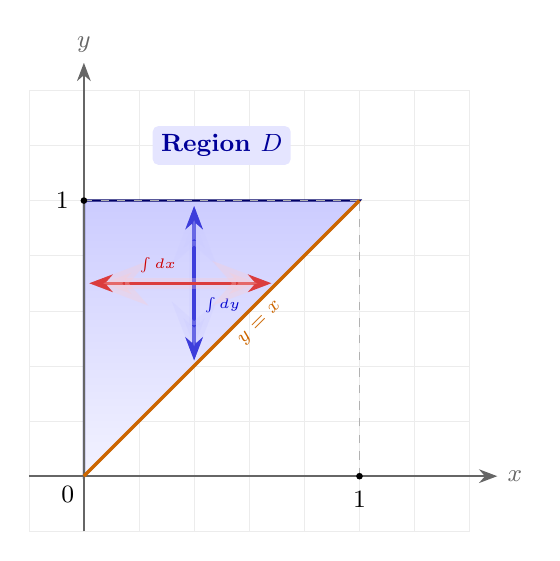
\begin{tikzpicture}[x=3.5cm, y=3.5cm, >=Stealth, font=\small] % 关键:设置单位长度为 3.5厘米

    % 1. 背景网格 (根据新单位调整范围,避免网格过大)
    \draw[very thin, gray!15, step=0.2] (-0.2,-0.2) grid (1.4, 1.4);
    
    % 2. 积分区域 D 的绘制 (比例会自动跟随单位缩放)
    \shade[top color=blue!20, bottom color=blue!5, draw=blue!40!black, thick] 
        (0,0) -- (1,1) -- (0,1) -- cycle;
    
    % 3. 坐标轴
    \draw[->, thick, gray!80!black] (-0.2,0) -- (1.5,0) node[right] {$x$};
    \draw[->, thick, gray!80!black] (0,-0.2) -- (0,1.5) node[above] {$y$};
    
    % 4. 边界线高亮
    \draw[dashed, gray!60] (1,0) -- (1,1);
    \draw[dashed, gray!60] (0,1) -- (1,1);
    \draw[very thick, orange!80!black] (0,0) -- (1,1) node[midway, below right, sloped, font=\scriptsize] {$y=x$};
    
    % 5. 扫描线 (发光质感)
    \draw[<->, blue!80!black, line width=1.2pt, postaction={draw, blue!20, line width=4pt, opacity=0.3}] 
        (0.4, 0.42) -- (0.4, 0.98) node[midway, right, yshift=-8pt, font=\tiny\bfseries] {$\int dy$};
        
    \draw[<->, red!80!black, line width=1.2pt, postaction={draw, red!20, line width=4pt, opacity=0.3}] 
        (0.02, 0.7) -- (0.68, 0.7) node[midway, above, xshift=-8pt, font=\tiny\bfseries] {$\int dx$};

    % 6. 装饰性标注
    \node[fill=blue!10, text=blue!60!black, rounded corners=2pt, inner sep=3pt, font=\small\bfseries] 
        at (0.5, 1.2) {Region $D$};
    
    % 7. 坐标刻度处理
    \node[below left] at (0,0) {$0$};
    \fill (1,0) circle (1.2pt) node[below=2pt] {$1$};
    \fill (0,1) circle (1.2pt) node[left=2pt] {$1$};

\end{tikzpicture}
\end{center}

\vspace{0.5em}
\textbf{二、 边缘概率密度 (Marginal Density)}
\begin{itemize}
    \item \textbf{公式}:$f_X(x) = \int_{-\infty}^{\infty} f(x,y) \, dy$ 以及 $f_Y(y) = \int_{-\infty}^{\infty} f(x,y) \, dx$。
    \item \textbf{注意}:求出的边缘分布必须注明自变量的取值范围(本题均为 $[0, 1]$),否则无法求出正确结果
\end{itemize}

\vspace{0.5em}
\textbf{三、 相关系数 $\rho(X,Y)$ 的计算步骤}
\begin{enumerate}
    \item \textbf{期望}:分别求出 $E(X)$、$E(Y)$ 以及混合矩 $E(XY) = \iint xy f(x,y) \, dx dy$。
    \item \textbf{协方差}:$\text{Cov}(X,Y) = E(XY) - E(X)E(Y)$。
    \item \textbf{方差}:计算 $\text{Var}(X)$ 和 $\text{Var}(Y)$。注意使用公式 $\text{Var}(X) = E(X^2) - [E(X)]^2$。
    \item \textbf{标准化}:相关系数是将协方差除以两个标准差的乘积,其值一定在 $[-1, 1]$ 之间。
\end{enumerate}

\vspace{0.5em}
\textbf{四、 需要注意的地方}
\begin{itemize}
    \item \textbf{计算过程}:积分计算易错,建议在求 $E(X^n)$ 时利用已知的边缘分布计算,比直接用联合分布进行二重积分更简便。
    \item \textbf{相关性判断}:若 $\rho = 0$,称 $X$ 与 $Y$ 不相关;本题 $\rho = 1/\sqrt{3} \approx 0.577$,说明两者存在正的线性相关关系。
\end{itemize}


    
\end{tcolorbox}

\textbf{Question 4: (7 marks)}

Let $X_1,\ldots,X_n$ constitute a random sample from the probability density function given by
\[
f_\theta(x)=
\begin{cases}
\dfrac{2}{\theta^2}(\theta - x), & 0 \le x \le \theta,\\[6pt]
0, & \text{elsewhere}.
\end{cases}
\]

Find an estimator for $\theta$ by using the method of moments.

{\color{blue}
\textbf{Solution to Question 4}

First, calculate $E(X)$:
\[
\begin{aligned}
E(X)
&= \int_0^\theta x \cdot \frac{2}{\theta^2}(\theta-x)\,dx \\
&= \frac{2}{\theta^2}\int_0^\theta (\theta x - x^2)\,dx \\
&= \frac{2}{\theta^2}\left[\frac{\theta x^2}{2}-\frac{x^3}{3}\right]_0^\theta \\
&= \frac{2}{\theta^2}\left(\frac{\theta^3}{2}-\frac{\theta^3}{3}\right) \\
&= \frac{\theta}{3}.
\end{aligned}
\]

Then equate $E(X)$ with the sample mean $\bar X$:
\[
\bar X = \frac{\theta}{3}.
\]

Finally, we get the result:
\[
\hat{\theta}_{\text{MM}} = 3\bar X.
\]
}

\begin{tcolorbox}[
        enhanced,
        colback=gray!10,
        colframe=black,
        width=\textwidth,
        arc=2mm, 
        auto outer arc,
        title={提示:矩估计法 (Method of Moments)},
        breakable
]

\textbf{一、 矩估计法的核心思想}
\begin{itemize}
    \item \textbf{基本原理}:利用样本的 $k$ 阶矩(如样本均值 $\bar{X}$)作为总体 $k$ 阶矩(如期望 $E(X)$)的估计量。
    \item \textbf{理论依据}:大数定律。当样本量 $n$ 足够大时,样本平均值依概率收敛于总体期望。
\end{itemize}

\vspace{0.5em}
\textbf{二、 解题步骤}
\begin{enumerate}
    \item \textbf{计算总体矩}:根据给定的概率密度函数 $f_\theta(x)$,计算期望 $E(X) = \int_{-\infty}^{+\infty} x f_\theta(x) \, dx$。此时结果通常是关于未知参数 $\theta$ 的函数。
    \item \textbf{建立方程}:令总体期望等于样本均值,即 $E(X) = \bar{X}$。
    \item \textbf{反解参数}:从方程中解出 $\theta$,得到的表达式即为矩估计量 $\hat{\theta}_{\text{MM}}$。
\end{enumerate}

\vspace{0.5em}
\textbf{三、 注意事项}
\begin{itemize}
    \item \textbf{积分区间}:在计算 $E(X)$ 时,务必注意分段函数的有效区间(本题为 $0$ 到 $\theta$),区间外的积分为 $0$。
    \item \textbf{多参数情况}:如果分布中有两个未知参数(如 $\mu$ 和 $\sigma^2$),则需要利用二阶矩,建立方程组:
    \[ \begin{cases} E(X) = \bar{X} \\ E(X^2) = \frac{1}{n}\sum X_i^2 \end{cases} \]
    \item \textbf{记号规范}:最终结果写成 $\hat{\theta}$,并在下标注明 MM (Method of Moments) 以示区分。
\end{itemize}

\end{tcolorbox}


\textbf{Question 5: (14 marks)}

The Rayleigh density function is given by
\[
f_\theta(x)=
\begin{cases}
\dfrac{2x}{\theta} e^{-x^2/\theta}, & x \ge 0,\\[6pt]
0, & \text{elsewhere}.
\end{cases}
\]

1. First show that $X^2$ has an exponential distribution with mean $\theta$; \\
2. If $X_1,\ldots,X_n$ denote a random sample from a Rayleigh distribution, find the MLE for $\theta$.

{\color{blue}
\textbf{Solution to Question 5}

1. Let $Y=X^2$. For $y>0$,
\[
\begin{aligned}
P(Y\le y)
&=P(X\le \sqrt y)
= \int_0^{\sqrt y} \frac{2x}{\theta}e^{-x^2/\theta}\,dx \\
&= \left[ -e^{-x^2/\theta} \right]_0^{\sqrt y} \\
&= 1-e^{-y/\theta}.
\end{aligned}
\]

Thus, the density of $Y$ is
\[
f_Y(y)=\frac{d}{dy}(1-e^{-y/\theta}) = \frac{1}{\theta}e^{-y/\theta}, \quad y>0,
\]
which is an exponential distribution with mean $\theta$.

2. Let $X_1,\ldots,X_n$ be a random sample. The likelihood function is
\[
L(\theta)=\prod_{i=1}^n \frac{2X_i}{\theta}e^{-X_i^2/\theta}.
\]

The log-likelihood is
\[
\ell(\theta)=n\ln2 + \sum_{i=1}^n \ln X_i - n\ln\theta -\frac{1}{\theta}\sum_{i=1}^n X_i^2.
\]

Differentiate with respect to $\theta$:
\[
\frac{d\ell}{d\theta} = -\frac{n}{\theta}+\frac{1}{\theta^2}\sum_{i=1}^n X_i^2.
\]

Setting this equal to zero gives
\[
\hat{\theta}_{\text{MLE}}=\frac{1}{n}\sum_{i=1}^n X_i^2.
\]
}

\begin{tcolorbox}[enhanced,
        colback=green!5!white, 
        colframe=green!60!black,
        width=\textwidth,
        arc=2mm, auto outer arc,
        title={提示:变量代换与极大似然估计},
        breakable]

\textbf{一、 变量代换法 (Transformation Method)}
\begin{itemize}
    \item \textbf{分布函数法}:求 $Y=g(X)$ 的分布时,先求其累积分布函数 $F_Y(y) = P(g(X) \le y)$,再求导得到密度函数 $f_Y(y)$。
    \item \textbf{识别分布}:得到 $f_Y(y) = \frac{1}{\theta}e^{-y/\theta}$ 后,应能立即识别出这是均值为 $\theta$ 的指数分布 $\text{Exp}(1/\theta)$。
\end{itemize}

\vspace{0.5em}
\textbf{二、 极大似然估计 (MLE) 的标准步骤}
\begin{enumerate}
    \item \textbf{写出似然函数 $L(\theta)$}:即所有观测值联合密度的乘积 $\prod_{i=1}^n f(x_i; \theta)$。
    \item \textbf{取对数 $\ell(\theta)$}:指数族分布(包含 $e$ 的函数)取对数后可以把乘法变加法,极大地简化求导过程。
    \item \textbf{求导并令其为零}:解似然方程 $\frac{d\ell}{d\theta} = 0$。
    \item \textbf{求出估计量 $\hat{\theta}$}:通常最后需要用样本观察值(如 $\sum X_i^2$)来表达 $\theta$。
\end{enumerate}

\vspace{0.5em}
\textbf{三、 注意事项}
\begin{itemize}
    \item \textbf{求导细节}:注意 $\frac{d}{d\theta}(-n\ln\theta) = -\frac{n}{\theta}$ 以及 $\frac{d}{d\theta}(-\frac{k}{\theta}) = \frac{k}{\theta^2}$ 的符号变化。
    \item \textbf{结果检查}:MLE 的结果通常与样本的某种“平均”形式相关。在本题中,由于 $X^2$ 的均值是 $\theta$,根据大数定律,$\theta$ 的估计量自然就是 $X^2$ 的样本均值 $\frac{1}{n}\sum X_i^2$。
\end{itemize}

\end{tcolorbox}

\textbf{Question 6: (14 marks)}

The specifications for a certain kind of ribbon call for a mean breaking strength of $185$ pounds and a standard deviation of $5$ pounds. Ten pieces randomly selected from different rolls have breaking strengths of
\[
171.6,\; 191.8,\; 178.3,\; 184.9,\; 189.1,\; 181.5,\; 176.4,\; 187.3,\; 190.7,\; 180.2
\]
pounds.

Under the assumption that the breaking strength is normally distributed as $N(\mu,\sigma^2)$, at a level of significance $0.05$, please determine whether the specifications for the mean and standard deviation are conformed.

{\color{blue}
\textbf{Solution to Question 6}

The specifications are
\[
\mu_0=185, \qquad \sigma_0=5.
\]

From the data above,
\[
\bar X = 183.37, \qquad S^2 = 39.56, \qquad n=10
\]

\textbf{1. Test for the mean}

Hypotheses: $H_0:\mu=185, \quad H_1:\mu\neq185$.

The test statistic is
\[
t=\frac{\bar X-\mu_0}{S/\sqrt n} =\frac{183.37-185}{\sqrt{39.56/10}} = -0.82.
\]

At significance level $0.05$, the critical value is $t_{0.025,9}=2.262$.

Since $|t|<2.262$, we fail to reject $H_0$. At the $5\%$ significance level, the mean specifications are conformed.

\textbf{2. Test for the variance}

Hypotheses: $H_0:\sigma^2=25, \quad H_1:\sigma^2\neq25$.

The test statistic is
\[
\chi^2=\frac{(n-1)S^2}{\sigma_0^2} =\frac{9\times 39.56}{25}=14.24.
\]

The critical values are $\chi^2_{0.025,9}=2.70$ and $\chi^2_{0.975,9}=19.02$.

Since $2.70 < 14.24 < 19.02$, we fail to reject $H_0$. At the $5\%$ significance level, the standard deviation specifications are conformed.
}


\begin{tcolorbox}[
    enhanced,
    colback=white,
    colframe=teal!60!black,
    arc=2mm,
    title={第6题:正态总体均值与方差的双侧检验},
    fonttitle=\bfseries,
    breakable,
    top=10pt,
    bottom=10pt
]

\textbf{【已知条件】} \\
规格要求:$\mu_0=185, \sigma_0=5$。样本量 $n=10$。\\
计算样本指标:平均值 $\bar{X} = 183.37$,样本方差 $S^2 = 39.56$。

\vspace{1em}
\textbf{一、 均值检验 ($t$ 检验)}
\begin{itemize}
    \item \textbf{建立假设}:$H_0: \mu = 185 \quad \text{vs} \quad H_1: \mu \neq 185$
    \item \textbf{计算统计量}:
    \[ t = \frac{\bar{X}-\mu_0}{S/\sqrt{n}} = \frac{183.37-185}{\sqrt{39.56/10}} \approx -0.82 \]
    \item \textbf{确定判定准则}:显著性水平 $\alpha=0.05$,自由度 $df=9$,查表得临界值 $t_{0.025}(9) = 2.262$。
\end{itemize}

\begin{center}
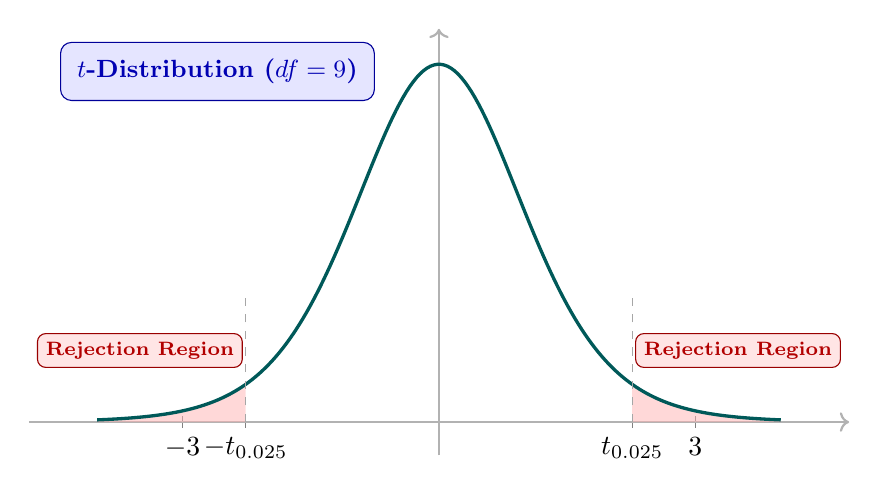
\begin{tikzpicture}
\begin{axis}[
    width=12cm,
    height=7cm,
    axis lines=middle,
    enlargelimits=true,
    samples=200,
    domain=-4:4,
    ytick=\empty,
    xtick={-3,-2.262,0,2.262,3},
    xticklabels={$-3$, $-t_{0.025}$, $0$, $t_{0.025}$, $3$},
    axis line style={->, thick, gray!60},
]

% =========================
% 1. t 分布曲线(df=9,形状近似)
% =========================
\addplot [
    name path=curve,
    very thick,
    teal!70!black
]
{1/(1 + x^2/9)^5};

% x 轴基线(用于填充)
\path [name path=axis] (axis cs:-4,0) -- (axis cs:4,0);

% =========================
% 2. 拒绝域填充
% =========================
% 左拒绝域
\addplot [
    fill=red!30,
    opacity=0.5
] fill between [
    of=curve and axis,
    soft clip={domain=-4:-2.262}
];

% 右拒绝域
\addplot [
    fill=red!30,
    opacity=0.5
] fill between [
    of=curve and axis,
    soft clip={domain=2.262:4}
];

% =========================
% 3. 临界值虚线
% =========================
\draw [dashed, gray!70] (axis cs:-2.262,0) -- (axis cs:-2.262,0.36);
\draw [dashed, gray!70] (axis cs:2.262,0) -- (axis cs:2.262,0.36);

% =========================
% 4. 顶部主标题(抬高到图外)
% =========================
\node[
    fill=blue!10,
    draw=blue!60!black,
    rounded corners=4pt,
    inner sep=6pt,
    font=\small\bfseries,
    text=blue!70!black
] 
at (rel axis cs:0.23,0.90)
{$t$-Distribution ($df=9$)};

% =========================
% 5. 左右拒绝域装饰性标注
% =========================
\node[
    fill=red!10,
    draw=red!60!black,
    rounded corners=3pt,
    inner sep=3pt,
    font=\scriptsize\bfseries,
    text=red!70!black
]
at (axis cs:-3.5,0.2)
{Rejection Region};

\node[
    fill=red!10,
    draw=red!60!black,
    rounded corners=3pt,
    inner sep=3pt,
    font=\scriptsize\bfseries,
    text=red!70!black
]
at (axis cs:3.5,0.2)
{Rejection Region};

\end{axis}
\end{tikzpicture}

\end{center}

\textbf{结论}:因为 $|t| = 0.82 < 2.262$,观测值落入接受域,故不拒绝 $H_0$。在 $5\%$ 显著水平下,均值符合规格。

\vspace{1.5em}
\textbf{二、 方差检验 ($\chi^2$ 检验)}
\begin{itemize}
    \item \textbf{建立假设}:$H_0: \sigma^2 = 25 \quad \text{vs} \quad H_1: \sigma^2 \neq 25$
    \item \textbf{计算统计量}:
    \[ \chi^2 = \frac{(n-1)S^2}{\sigma_0^2} = \frac{9 \times 39.56}{25} \approx 14.24 \]
    \item \textbf{确定判定准则}:显著性水平 $\alpha=0.05$。查表得临界值:\\
    左侧 $\chi^2_{0.975}(9) = 2.70$,右侧 $\chi^2_{0.025}(9) = 19.02$。
\end{itemize}

\begin{center}
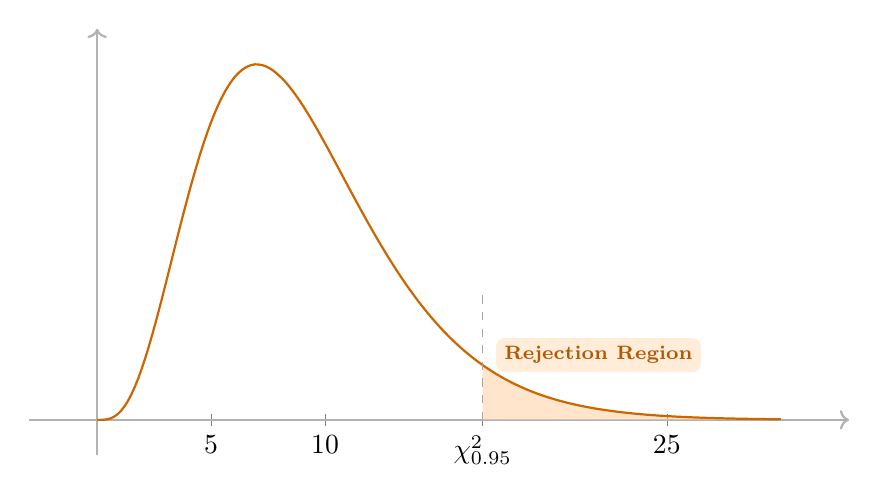
\begin{tikzpicture}
\begin{axis}[
    width=12cm, height=7cm,
    axis lines=middle,
    enlargelimits=true,
    samples=200,
    domain=0:30,
    ytick=\empty,
    xtick={0,5,10,16.92,25},
    xticklabels={$0$, $5$, $10$, $\chi^2_{0.95}$, $25$},
    axis line style={->, thick, gray!60},
]

% =========================
% 1. 卡方分布曲线(df=9,形状比例化)
% =========================
\addplot [
    name path=curve,
    thick,
    orange!80!black
] {0.05 * x^3.5 * exp(-x/2)};

% x 轴基线
\path [name path=axis] (axis cs:0,0) -- (axis cs:30,0);

% =========================
% 2. 右尾拒绝域(渐变质感)
% =========================
\addplot [
    fill=orange!40,
    opacity=0.5
] fill between [
    of=curve and axis,
    soft clip={domain=16.92:30}
];

% =========================
% 3. 临界值虚线
% =========================
\draw [dashed, gray!70] 
    (axis cs:16.92,0) -- (axis cs:16.92,0.48);

% =========================
% 4. 装饰性标题(放在图上方)
% =========================
\node[
    fill=orange!10,
    draw=orange!70!black,
    rounded corners=4pt,
    inner sep=6pt,
    font=\small\bfseries,
    text=orange!80!black
] 
at (rel axis cs:10,0.45)
{$\chi^2$-Distribution ($df=9$)};

% =========================
% 5. 装饰性拒绝域标注
% =========================
\node[
    fill=orange!15,
    rounded corners=3pt,
    inner sep=3pt,
    font=\scriptsize\bfseries,
    text=orange!70!black
] at (axis cs:22,0.25)
{Rejection Region};

\end{axis}
\end{tikzpicture}
\end{center}


\textbf{结论}:因为 $2.70 < 14.24 < 19.02$,统计量落入接受域,故不拒绝 $H_0$。方差亦符合规格。

\end{tcolorbox}

\newpage
\begin{center}
\large{\textbf{BDIC2005J Probability and Statistics 2018-2019}}
\end{center}

\noindent \textbf{Question 1:} \\
\textbf{Vacancy (Each blank 3 marks)}

\vspace{1em}

(1). There are two events $A$ and $B$. $P(A)=0.1, P(A \cup B)=0.4$. 
    
If $A$ and $B$ are mutually exclusive, $P(B) = $. 
 
If $A$ and $B$ are \colorbox{white}{mutually independent}, $P(B) = $.

{\color{blue}
\textbf{Solution:}

For mutually exclusive events,
\[
P(A\cup B)=P(A)+P(B).
\]

Thus,
\[
0.4 = 0.1 + P(B),
\]

which gives
\[
P(B)=0.3
\]

For independent events,
\[
P(A\cap B)=P(A)P(B).
\]

Using the union formula,
\[
P(A\cup B)=P(A)+P(B)-P(A\cap B),
\]

we have
\[
0.4 = 0.1 + P(B) - 0.1P(B).
\]

Hence,
\[
0.4 = 0.1 + 0.9P(B),
\]
\[
0.9P(B)=0.3,
\]
and therefore
\[
P(B)=\frac{1}{3}
\]
}

\begin{tcolorbox}[
        enhanced,
        colback=blue!5,
        colframe=blue!50!black,
        width=\textwidth,
        arc=2mm, 
        auto outer arc,
        title={考点:“互斥”和“独立”},
        breakable
]

\textbf{1. 核心考点:两种关系的本质区别}
\begin{itemize}
    \item \textbf{互斥 (Mutually Exclusive)}:两个事件“有你没我”,不能同时发生,所以交集 $P(AB) = 0$。计算并集时直接求和即可:$P(A \cup B) = P(A) + P(B)$。
    \item \textbf{独立 (Independent)}:指的是两个事件“互不干涉”,一个发不发生不影响另一个。此时交集的概率等于概率的乘积:$P(AB) = P(A)P(B)$。
\end{itemize}



\vspace{0.5em}
\textbf{2. 易错点}
\begin{itemize}
    \item \textbf{减项}:在处理独立事件时,牢记并集公式 $P(A \cup B) = P(A) + P(B) - P(AB)$ 后面那个减项。只有互斥时那个减项才为 0。
    \item \textbf{代数计算}:独立情况下的方程 $0.4 = 0.1 + P(B) - 0.1P(B)$,可以看作是 $0.3 = (1 - 0.1)P(B)$。解方程时别在小数点上栽跟头。
\end{itemize}

\vspace{0.5em}
\textbf{3. 解题技巧}
\begin{itemize}
    \item 看到“互斥”, $P(AB)=0$。
    \item 看到“独立”, $P(AB)=P(A)P(B)$。
    \item 无论哪种情况,通用的并集公式 $P(A \cup B) = P(A) + P(B) - P(AB)$ 。
\end{itemize}

\end{tcolorbox}
(2). Suppose the random variable $X \sim U(a, b)$. $E(X)=5, D(X)=3$, $a = , b = $.

{\color{blue}
\textbf{Solution:}

For a uniform distribution,
\[
E(X)=\frac{a+b}{2}, \quad D(X)=\frac{(b-a)^2}{12}.
\]

From the expectation,
\[
\frac{a+b}{2}=5 \Rightarrow a+b=10.
\]

From the variance,
\[
\frac{(b-a)^2}{12}=3 \Rightarrow (b-a)^2=36,
\]
which implies
\[
b-a=6.
\]

Solving the system,
\[
\begin{cases}
a+b=10, \\
b-a=6,
\end{cases}
\]
we obtain
\[
a=2,\quad b=8
\]
}

\begin{tcolorbox}[
        enhanced,
        colback=orange!5,
        colframe=orange!50!black,
        width=\textwidth,
        arc=2mm, 
        auto outer arc,
        title={考点:均匀分布},
        breakable
]

\textbf{1. 核心公式}
\begin{itemize}
    \item \textbf{均值 (Expectation)}:$E(X) = \frac{a+b}{2}$。直观理解就是区间的“中点”。
    \item \textbf{方差 (Variance)}:$D(X) = \frac{(b-a)^2}{12}$。容易记混的地方:分母是 $12$,分子是区间长度的平方。
\end{itemize}

\vspace{0.5em}
\textbf{2. 易错点}
\begin{itemize}
    \item \textbf{开方}:计算 $(b-a)^2 = 36$ 时,虽然代数上有 $\pm 6$ 两种可能,但根据均匀分布定义,上界 $b$ 一定大于下界 $a$,所以直接取 $b-a=6$ 即可。
    \item \textbf{公式}:别把方差的分母记成 $2$ 或者 $4$。
\end{itemize}

\vspace{0.5em}
\textbf{3. 解题技巧}
\begin{itemize}
    \item 这类题本质上是“解二元一次方程组”。
    \item 第一步:根据均值算出 $a+b$。
    \item 第二步:根据方差算出 $b-a$。
\end{itemize}

\end{tcolorbox}

(3). Let $X_1, X_2, \cdots, X_n (n > 2)$ be a sample from $N(\mu, \sigma^2)$.
\[
\bar{X} = \frac{1}{n} \sum_{i=1}^n X_i, \quad S^2 = \frac{1}{n-1} \sum_{i=1}^n (X_i - \bar{X})^2 .
\]
$\sqrt{n}(\bar{X} - \mu) / \sqrt{S^2} \sim , \quad (n-1)S^2 / \sigma^2 \sim $.

{\color{blue}
\textbf{Solution:}
\[
\frac{\sqrt{n}(\bar X-\mu)}{S}\sim t_{n-1},
\]
and
\[
\frac{(n-1)S^2}{\sigma^2}\sim \chi^2_{n-1}.
\]
}

\begin{tcolorbox}[
        enhanced,
        colback=purple!5,
        colframe=purple!50!black,
        width=\textwidth,
        arc=2mm, 
        auto outer arc,
        title={考点:数理统计的三大分布},
        breakable
]

\textbf{1. 核心考点:由正态分布衍生的分布}
\begin{itemize}
    \item \textbf{卡方分布 ($\chi^2$)}:用来描述“方差”的分布。公式 $\frac{(n-1)S^2}{\sigma^2} \sim \chi^2_{n-1}$。这里的自由度是 $n-1$,因为在计算 $S^2$ 时掉了一个自由度(用掉了样本均值 $\bar{X}$)。
    \item \textbf{$t$ 分布}:当总体方差 $\sigma^2$ 未知,我们被迫用样本方差 $S^2$ 来代替它时,原本的正态分布就变成了 $t$ 分布。公式为 $\frac{\bar{X}-\mu}{S/\sqrt{n}} \sim t_{n-1}$。
\end{itemize}



\vspace{0.5em}
\textbf{2. 易错点}
\begin{itemize}
    \item \textbf{对应关系}:记住“方差比方差”通常对应卡方;“均值比标准差”通常对应 $t$ 分布。
    \item \textbf{自由度}:这两个统计量的自由度都是 $n-1$,千万不要手抖写成 $n$。
    \item \textbf{符号}:注意 $t$ 分布公式里分母是 $S$(样本标准差),而卡方公式里是 $S^2$(样本方差)。
\end{itemize}

\vspace{0.5em}
\textbf{3. 解题技巧}
\begin{itemize}
    \item  $\sqrt{n}$ 出现在分子上,且分母有 $S$ 的,是 $t$ 分布。
    \item 有 $(n-1)S^2$ 这种的,是 $\chi^2$ 分布。
    \item \textbf{记忆}:$t$ 分布是胖的正态分布”,随着 $n$ 变大,它会越来越像标准正态分布 $N(0,1)$。
\end{itemize}

\end{tcolorbox}

(4). Let $X_1, \cdots, X_{10}$ be a sample from $N(\mu, \sigma^2)$. We can calculate the sample mean $5$ and sample variance $0.25$ are respectively. $\mu$ and $\sigma^2$ are unknown parameters. 
    
The confidence interval of $\mu$ with confidence level $95\%$ is $[, ]$. 
    
The confidence interval of $\sigma^2$ with confidence level $95\%$ is $[, ]$.

{\color{blue}
\textbf{Solution:}

Since $\sigma^2$ is unknown, the $95\%$ confidence interval for $\mu$ is
\[
\bar X \pm t_{0.975}(n-1)\frac{S}{\sqrt n}.
\]

With $t_{0.975}(9)=2.262$ and $S=0.5$,
\[
\frac{S}{\sqrt n}=\frac{0.5}{\sqrt{10}}.
\]

Thus, the confidence interval is
\[
[\,4.643,\;5.357\,]
\]

The $95\%$ confidence interval for $\sigma^2$ is
\[
\left[
\frac{(n-1)S^2}{\chi^2_{0.975}(n-1)},
\frac{(n-1)S^2}{\chi^2_{0.025}(n-1)}
\right].
\]

Using $\chi^2_{0.975}(9)=19.023$ and $\chi^2_{0.025}(9)=2.700$,
\[
(n-1)S^2=9\times0.25=2.25.
\]

Therefore, the confidence interval is
\[
[\,0.118,\;0.833\,]
\]
}

\begin{tcolorbox}[
        enhanced,
        colback=green!5,
        colframe=green!50!black,
        width=\textwidth,
        arc=2mm, 
        auto outer arc,
        title={核心要点:单正态总体的区间估计},
        breakable
]

\textbf{1. 均值 $\mu$ 的置信区间($\sigma^2$ 未知)}
\begin{itemize}
    \item \textbf{核心公式}:$\left[ \bar{X} - t_{\alpha/2}(n-1)\frac{S}{\sqrt{n}}, \bar{X} + t_{\alpha/2}(n-1)\frac{S}{\sqrt{n}} \right]$。
    \item \textbf{关键点}:因为总体方差 $\sigma^2$ 未知,必须使用 $t$ 分布。注意分母使用的是样本标准差 $S$ 而非方差 $S^2$。
\end{itemize}



\vspace{0.5em}
\textbf{2. 方差 $\sigma^2$ 的置信区间}
\begin{itemize}
    \item \textbf{核心公式}:$\left[ \frac{(n-1)S^2}{\chi^2_{\alpha/2}(n-1)}, \frac{(n-1)S^2}{\chi^2_{1-\alpha/2}(n-1)} \right]$。
    \item \textbf{注意}:卡方分布是非对称的,因此区间的左端点对应较大的分位数(分母大,数值小),右端点对应较小的分位数。
\end{itemize}

\vspace{0.5em}
\textbf{3. 易错点提醒}
\begin{itemize}
    \item \textbf{查表分位数}:置信水平为 $95\%$ 时,对应双侧显著性水平 $\alpha = 0.05$,查表时应找 $\alpha/2 = 0.025$ 或 $1-\alpha/2 = 0.975$ 对应的数值。
    \item \textbf{样本标准差与方差}:题目给出的“样本方差 $0.25$”是 $S^2$,计算均值区间时要记得开方取 $S = 0.5$。
    \item \textbf{自由度 $n-1$}:本题样本量 $n=10$,所有查表操作均需基于自由度 $df = 9$。
\end{itemize}

\end{tcolorbox}

\textbf{Question 2: (14 marks)}

$5$ of the $8$ guns have been calibrated, $3$ have not been calibrated. The probability of a shooter hitting a target with a calibrated gun is $0.8$; The probability of the shooter hitting target using an uncalibrated gun is $0.3$.\\
(a) Find the probability of the shooter not hitting target;\\
(b) Now take one of the $8$ guns and shoot, the result is that the shooter hits the target. Find the probability that the gun used to shoot is a calibrated gun.

{\color{blue}
\textbf{Solution:}

There are $8$ guns in total, among which $5$ are calibrated and $3$ are uncalibrated.
The probability that the shooter hits the target using
\begin{itemize}
\item a calibrated gun is $0.8$,
\item an uncalibrated gun is $0.3$.
\end{itemize}

\textbf{(a) Probability that the shooter does not hit the target}

First, compute the probability of choosing each type of gun:
\[
P(C)=\frac{5}{8}, \quad P(U)=\frac{3}{8}.
\]

The probability of missing the target given each gun type is
\[
P(M \mid C)=1-0.8=0.2, \quad P(M \mid U)=1-0.3=0.7.
\]

By the law of total probability,
\[
P(M)=P(M\mid C)P(C)+P(M\mid U)P(U).
\]

Thus,
\[
P(M)=0.2\cdot\frac{5}{8}+0.7\cdot\frac{3}{8}
=\frac{1}{8}+\frac{2.1}{8}
=\frac{3.1}{8}.
\]

\[
P(\text{not hit})=\frac{3.1}{8}
\]


\textbf{(b) Probability that the gun is calibrated given a hit}

Let $H$ denote the event that the target is hit.

First compute $P(H)$:
\[
P(H)=P(H\mid C)P(C)+P(H\mid U)P(U)
=0.8\cdot\frac{5}{8}+0.3\cdot\frac{3}{8}
=\frac{4.9}{8}.
\]

Using Bayes' theorem,
\[
P(C\mid H)=\frac{P(H\mid C)P(C)}{P(H)}
=\frac{0.8\cdot\frac{5}{8}}{\frac{4.9}{8}}
=\frac{4}{4.9}.
\]

\[
P(C\mid H)=\frac{4}{4.9}
\]
}

\begin{tcolorbox}[
        enhanced,
        colback=blue!5,
        colframe=blue!50!black,
        width=\textwidth,
        arc=2mm, 
        auto outer arc,
        title={核心要点:全概率公式与贝叶斯推断},
        breakable
]

\textbf{1. 知识点定位:分阶段概率模型}
\begin{itemize}
    \item \textbf{全概率公式}:用于计算“结果”的总概率。当一个事件(如“没击中”)可以通过多种途径(如“用校准枪”或“用未校准枪”)发生时,我们需要加权求和。
    \item \textbf{贝叶斯定理}:用于“由果溯因”。在已知结果发生的条件下,计算它是由某个特定原因引起的概率。
\end{itemize}



\vspace{0.5em}
\textbf{2. 解题逻辑梳理}
\begin{itemize}
    \item \textbf{第一步:理清概率树}。
    \begin{itemize}
        \item 第一层:选枪。$P(C) = 5/8$,$P(U) = 3/8$。
        \item 第二层:射击结果。注意“击中”与“未击中”互为对立事件。
    \end{itemize}
    \item \textbf{第二步:对立事件的应用}。在第(a)问中,已知击中概率为 $0.8$,则未击中概率 $P(M|C) = 1 - 0.8 = 0.2$。
    \item \textbf{第三步:分母是对子集的汇总}。在第(b)问使用贝叶斯公式时,分母 $P(H)$ 实际上是所有能导致“击中”的路径概率之和。
\end{itemize}

\vspace{0.5em}
\textbf{3. 易错点提醒}
\begin{itemize}
    \item \textbf{事件定义模糊}:建议在草稿纸上明确列出 $C$(校准枪)、$U$(未校准枪)、$H$(击中)等符号,避免计算时将概率放错位置。
    \item \textbf{忽视互斥性}:全概率公式的前提是各种原因(校准与未校准)必须是互斥且构成完备事件组的(即枪只有这两类)。
    \item \textbf{计算陷阱}:最后的计算结果(如 $4/4.9$)可以化简为 $40/49$。在概率题中,分数形式通常比小数更精确。
\end{itemize}

\end{tcolorbox}

% --- Question 3 
\textbf{Question 3: (14 marks)}

Suppose that the probability density function of the continuous random variable $X$ is
\[
f(x) = 
\begin{cases} 
\dfrac{1}{c^2 + x^2}, & x \in (0, \dfrac{\pi}{4}); \\
0, & \text{elsewhere}.
\end{cases}
\]

Find:\\
(a) \quad The value of constant $c$;\\
(b) \quad $P \left( \dfrac{\sqrt{3}\pi}{12} < X \le \dfrac{\pi}{3} \right)$;\\
(c) \quad $E(X)$.


{\color{blue}
\textbf{Solution:}

\textbf{(a) Determination of constant $c$}

Since $f(x)$ is a probability density function, it must satisfy
\[
\int_0^{\pi/4} \frac{1}{c^2+x^2}\,dx=1.
\]

Recall that
\[
\int \frac{1}{c^2+x^2}\,dx=\frac{1}{c}\arctan\left(\frac{x}{c}\right).
\]

Therefore,
\[
\frac{1}{c}\left[\arctan\left(\frac{x}{c}\right)\right]_0^{\pi/4}=1,
\]
which gives
\[
\frac{1}{c}\arctan\left(\frac{\pi}{4c}\right)=1.
\]

Hence,
\[
\arctan\left(\frac{\pi}{4c}\right)=c
\]



\textbf{(b) Probability $\displaystyle P\left(\frac{\sqrt{3}\pi}{12}<X\le\frac{\pi}{3}\right)$}

Since the support of $X$ is $\left(0,\frac{\pi}{4}\right)$, note that
\[
\frac{\pi}{3}>\frac{\pi}{4}.
\]

Thus,
\[
P\left(\frac{\sqrt{3}\pi}{12}<X\le\frac{\pi}{3}\right)
= P\left(\frac{\sqrt{3}\pi}{12}<X\le\frac{\pi}{4}\right).
\]

Compute the probability:
\[
\int_{\frac{\sqrt{3}\pi}{12}}^{\frac{\pi}{4}} \frac{1}{c^2+x^2}\,dx
= \frac{1}{c}\left[
\arctan\left(\frac{x}{c}\right)
\right]_{\frac{\sqrt{3}\pi}{12}}^{\frac{\pi}{4}}.
\]

Thus,
\[
P=\frac{1}{c}
\left[
\arctan\left(\frac{\pi}{4c}\right)
-\arctan\left(\frac{\sqrt{3}\pi}{12c}\right)
\right]
\]



\textbf{(c) Expectation $E(X)$}

The expectation of $X$ is
\[
E(X)=\int_0^{\pi/4} x f(x)\,dx
=\int_0^{\pi/4} \frac{x}{c^2+x^2}\,dx.
\]

Using the substitution $u=c^2+x^2$, we obtain
\[
\int \frac{x}{c^2+x^2}\,dx
=\frac{1}{2}\ln(c^2+x^2).
\]

Therefore,
\[
E(X)=\frac{1}{2}\left[
\ln(c^2+x^2)
\right]_0^{\pi/4}
=\frac{1}{2}\ln\left(\frac{c^2+\left(\frac{\pi}{4}\right)^2}{c^2}\right).
\]

\[
E(X)=\frac{1}{2}\ln\left(1+\frac{\pi^2}{16c^2}\right)
\]
}

\begin{tcolorbox}[
        enhanced,
        colback=red!5,
        colframe=red!50!black,
        width=\textwidth,
        arc=2mm, 
        auto outer arc,
        title={核心要点:连续型随机变量的微积分应用},
        breakable
]

\textbf{1. 知识点定位:密度函数}
\begin{itemize}
    \item \textbf{归一化}:PDF 在整个实数域上的积分必须等于 $1$。在解决第 (a) 问时,这是确定待定系数 $c$ 的唯一途径。
    \item \textbf{概率是面积}:连续型随机变量在某个区间内的概率,等于该区间上密度函数的定积分。
    \item \textbf{期望的定义}:$E(X) = \int_{-\infty}^{+\infty} x f(x) \, dx$。可以形象地理解为所有可能取值 $x$ 与其对应概率密度 $f(x)$ 的加权平均积分。
\end{itemize}



\vspace{0.5em}
\textbf{2. 微积分}
\begin{itemize}
    \item \textbf{反三角函数积分}:本题涉及 $\int \frac{1}{c^2+x^2} dx = \frac{1}{c} \arctan(\frac{x}{c}) + C$。这是考试中涉及 PDF 性质时的常见积分形式。
    \item \textbf{换元积分法}:在计算期望时,分子出现了 $x$,此时应联想到使用对数积分形式:$\int \frac{x}{c^2+x^2} dx = \frac{1}{2} \ln(c^2+x^2) + C$。
\end{itemize}

\vspace{0.5em}
\textbf{3. 易错点}
\begin{itemize}
    \item \textbf{有效区间判定}:在第 (b) 问中,题目给出的上限 $\pi/3$ 超过了密度函数的定义域上限 $\pi/4$。切记:在定义域之外 $f(x) = 0$,积分时只需计算到 $\pi/4$ 即可。
    \item \textbf{参数 $c$ 的隐函数形式}:第 (a) 问解出的 $c$ 满足 $\arctan(\frac{\pi}{4c}) = c$。在没有具体数值表的情况下,后续步骤通常保留 $c$ 的表达式,不需要强行求出数值解。
    \item \textbf{期望计算漏掉 $x$}:计算 $E(X)$ 时,积分表达式是 $x \cdot f(x)$,不要直接对 $f(x)$ 求积分(那样结果永远是 $1$)。
\end{itemize}

\end{tcolorbox}

% --- Question 4 ---
\textbf{Question 4: (14 marks)}

Suppose that the joint probability density of two random variables $X$ and $Y$ are given by
\[ f(x, y) = \begin{cases} 
c \cdot y^3(2-x), & 0 \leq x \leq 1, 0 \leq y \leq x, \\
0, & \text{elsewhere.}
\end{cases} \]
Find:

(a)The value of constant $c$;

(b)The marginal densities $f_X(x), f_Y(y)$;

(c)Whether the two random variables $X$ and $Y$ are independent or not? (Please 
give your reason);

(d)$E(XY)$

{\color{blue}
\textbf{Solution:}

The joint probability density function of $(X,Y)$ is
\[
f(x,y)=
\begin{cases}
c\,y^3(2-x), & 0\le x\le1,\;0\le y\le x,\\
0, & \text{elsewhere}.
\end{cases}
\]

\textbf{(a) Determination of constant $c$}

Since $f(x,y)$ is a joint pdf,
\[
\int_0^1 \int_0^x c\,y^3(2-x)\,dy\,dx = 1.
\]

Compute the inner integral:
\[
\int_0^x y^3\,dy = \frac{x^4}{4}.
\]

Thus,
\[
c \int_0^1 (2-x)\frac{x^4}{4}\,dx = 1.
\]

\[
\frac{c}{4}\int_0^1 (2x^4-x^5)\,dx
= \frac{c}{4}\left(\frac{2}{5}-\frac{1}{6}\right)
= \frac{c}{4}\cdot\frac{7}{30}.
\]

Hence,
\[
\frac{7c}{120}=1 \Rightarrow c=\frac{120}{7}
\]

\bigskip

\textbf{(b) Marginal densities}

\textbf{Marginal density of $X$:}
\[
f_X(x)=\int_0^x c\,y^3(2-x)\,dy
= c(2-x)\frac{x^4}{4},
\quad 0\le x\le1.
\]

\[
f_X(x)=\frac{30}{7}x^4(2-x), \; 0\le x\le1
\]

\textbf{Marginal density of $Y$:}

For fixed $y$, $x$ ranges from $y$ to $1$:
\[
f_Y(y)=\int_y^1 c\,y^3(2-x)\,dx.
\]

\[
= c y^3\left[2x-\frac{x^2}{2}\right]_y^1
= c y^3\left(\frac{3}{2}-2y+\frac{y^2}{2}\right).
\]

\[
f_Y(y)=\frac{120}{7}y^3\left(\frac{3}{2}-2y+\frac{y^2}{2}\right),
\; 0\le y\le1
\]

\bigskip

\textbf{(c) Independence of $X$ and $Y$}

If $X$ and $Y$ were independent, then
\[
f(x,y)=f_X(x)f_Y(y).
\]

However, the support of $(X,Y)$ satisfies $0\le y\le x$, which is not a rectangular region.
Therefore, $X$ and $Y$ are \textbf{not independent}.

\[
X \text{ and } Y \text{ are not independent}
\]

\bigskip

\textbf{(d) Computation of $E(XY)$}

\[
E(XY)=\int_0^1 \int_0^x xy\,c\,y^3(2-x)\,dy\,dx.
\]

\[
= c\int_0^1 x(2-x)\int_0^x y^4\,dy\,dx
= c\int_0^1 x(2-x)\frac{x^5}{5}\,dx.
\]

\[
= \frac{c}{5}\int_0^1 (2x^6-x^7)\,dx
= \frac{c}{5}\left(\frac{2}{7}-\frac{1}{8}\right)
= \frac{c}{5}\cdot\frac{9}{56}.
\]

Substitute $c=\frac{120}{7}$:
\[
E(XY)=\frac{108}{245}
\]
}

\begin{tcolorbox}[
        enhanced,
        colback=yellow!5,
        colframe=yellow!50!black,
        width=\textwidth,
        arc=2mm, 
        auto outer arc,
        title={核心要点:二维随机变量的综合分析},
        breakable
]

\textbf{1. 知识点定位:从“面”到“线”的转化}
\begin{itemize}
    \item \textbf{联合密度的归一性}:在二维平面区域上,联合概率密度函数 $f(x,y)$ 的二重积分必须等于 $1$。这是求常数 $c$ 的基本依据。
    \item \textbf{边缘分布 (Marginal Density)}:求 $X$ 的边缘分布时,“积掉” $y$;求 $Y$ 的边缘分布时,“积掉” $x$。
    \item \textbf{独立性判定}:
    \begin{itemize}
        \item \textbf{代数标准}:看是否满足 $f(x,y) = f_X(x) \cdot f_Y(y)$。
        \item \textbf{几何直观}:如果变量的取值范围(支撑集)不是一个**矩形区域**(如本题中 $y$ 的范围依赖于 $x$),那么这两个变量通常不独立。
    \end{itemize}
\end{itemize}

\vspace{0.5em}
\textbf{2. 关键难点:确定积分上下限}



\begin{itemize}
    \item \textbf{求 $f_X(x)$}:固定 $x$,观察 $y$ 的变动范围。根据题目条件 $0 \le y \le x$,积分限即为 $0$ 到 $x$。
    \item \textbf{求 $f_Y(y)$}:固定 $y$,观察 $x$ 的变动范围。从区域图中可以看出,对于确定的 $y$,$x$ 是从直线 $x=y$ 开始变到 $x=1$ 为止。因此积分限是 $y$ 到 $1$。这是本题最易出错的地方。
\end{itemize}

\vspace{0.5em}
\textbf{3. 计算建议与提醒}
\begin{itemize}
    \item \textbf{分步积分}:处理 $E(XY)$ 这种复杂的二重积分时,先对其中一个变量求内层积分,化简后再对第二个变量积分,避免算式过于臃肿。
    \item \textbf{结果自检}:边缘分布 $f_X(x)$ 和 $f_Y(y)$ 本身也是概率密度函数,它们在各自区间上的积分也必须等于 $1$。如果时间充裕,可以通过这个方法校验计算是否正确。
\end{itemize}

\end{tcolorbox}


% --- Question 5 ---
\textbf{Question 5: (14 marks)}

Suppose $X_1, X_2 \cdots X_n$ is a sample from $X$, and the probability density function of $X$ is
\[ f(x; \theta) = \begin{cases} 
\theta^2 x e^{-\theta x}, & x > 0, \\
0, & x \leq 0,
\end{cases} \]
where $\theta > 0$. Find:

(a) The moment estimator of $\theta$;

(b) The maximum likelihood estimator of $\theta$.

{\color{blue}
\textbf{Solution:}

\textbf{(a) Moment estimator of $\theta$}

Compute the expectation:
\[
E(X)=\int_0^\infty x\theta^2 x e^{-\theta x}\,dx
=\theta^2\int_0^\infty x^2 e^{-\theta x}\,dx.
\]

Using $\int_0^\infty x^2 e^{-\theta x}\,dx=\frac{2}{\theta^3}$,
\[
E(X)=\frac{2}{\theta}.
\]

Equating $E(X)$ with the sample mean $\bar X$,
\[
\bar X=\frac{2}{\theta}
\Rightarrow
\hat\theta_{\text{MM}}=\frac{2}{\bar X}
\]

\bigskip

\textbf{(b) Maximum likelihood estimator of $\theta$}

The likelihood function is
\[
L(\theta)=\prod_{i=1}^n \theta^2 X_i e^{-\theta X_i}
=\theta^{2n}\left(\prod X_i\right)e^{-\theta\sum X_i}.
\]

The log-likelihood is
\[
\ell(\theta)=2n\ln\theta+\sum\ln X_i-\theta\sum X_i.
\]

Differentiate and set equal to zero:
\[
\frac{d\ell}{d\theta}=\frac{2n}{\theta}-\sum X_i=0.
\]

Thus,
\[
\hat\theta_{\text{MLE}}=\frac{2n}{\sum X_i}
\]
}

\begin{tcolorbox}[
        enhanced,
        colback=cyan!5,
        colframe=cyan!50!black,
        width=\textwidth,
        arc=2mm, 
        auto outer arc,
        title={核心要点:矩估计与极大似然估计},
        breakable
]

\textbf{1. 知识点定位:参数估计的两种方法}
\begin{itemize}
    \item \textbf{矩估计法 (Method of Moments)}:核心思想是用“样本矩”去估计“总体矩”。通常第一步是计算总体均值 $E(X)$(即一阶原点矩),然后令 $E(X) = \bar{X}$,解出未知参数。
    \item \textbf{极大似然估计法 (MLE)}:核心思想是寻找一个参数值 $\theta$,使得当前观测到的样本序列出现的概率(似然度)达到最大。
\end{itemize}

\vspace{0.5em}
\textbf{2. 解题步骤与技巧}
\begin{itemize}
    \item \textbf{矩估计中的积分计算}:计算 $E(X)$ 时,常涉及形如 $\int_0^\infty x^n e^{-ax} dx$ 的积分,这与 $\Gamma$ 函数相关。记住结论 $\int_0^\infty x^n e^{-\theta x} dx = \frac{n!}{\theta^{n+1}}$ 可以大幅提高计算速度。
    \item \textbf{极大似然的标准三部曲}:
    \begin{enumerate}
        \item 写出似然函数 $L(\theta)$(所有样本密度的乘积)。
        \item 取对数得到 $\ln L(\theta)$(将连乘变连加,方便求导)。
        \item 求导并令导数为 $0$,解方程得到 $\hat{\theta}$。
    \end{enumerate}
\end{itemize}



\vspace{0.5em}
\textbf{3. 易错点}
\begin{itemize}
    \item \textbf{指数项处理}:在极大似然估计中,$\prod e^{-\theta X_i}$ 应该化简为 $e^{-\theta \sum X_i}$。对数化后,它会变成 $-\theta \sum X_i$,求导后只剩下 $-\sum X_i$。
    \item \textbf{参数位置}:注意本题中参数 $\theta$ 在底数和指数位置同时出现。在对数似然函数中,$\ln(\theta^{2n})$ 应写成 $2n \ln \theta$。
    \item \textbf{合理性检查}:在大多数简单分布中,矩估计和极大似然估计的结果往往形式相似(如本题中均与 $2/\bar{X}$ 相关),如果两个结果差异巨大,建议回头检查计算。
\end{itemize}

\end{tcolorbox}


% --- Question 6 ---
\textbf{Question 6: (14 marks)}

The capacities (in ampere-hours) of 10 batteries were recorded as follows:
\[ 102, 97, 101, 103, 101, 98, 99, 104, 103, 98 \]
Under the assumption that the capacity is normal distributed as $N(\mu, \sigma^2)$.\\
Question: at level of significance 0.05,

(a)test $H_0 : \mu = 100 \leftrightarrow H_1 : \mu \neq 100$, \quad (b) test $H_0 : \sigma^2 = 2.5 \leftrightarrow H_1 : \sigma^2 > 2.5$.


\begin{center}
The $t$ distribution table and the $\chi^2$ distribution table
\begin{tabular}{|l|l|l|l|}
\hline
$t_9(0.025) = 2.2622$ & $t_9(0.05) = 1.8331$ & $t_{10}(0.025) = 2.2281$ & $t_{10}(0.05) = 1.8125$ \\ \hline
$\chi^2_9(0.025) = 19.023$ & $\chi^2_9(0.05) = 16.919$ & $\chi^2_9(0.975) = 2.700$ & $\chi^2_9(0.95) = 3.325$ \\ \hline
$\chi^2_{10}(0.025) = 20.483$ & $\chi^2_{10}(0.05) = 18.307$ & $\chi^2_{10}(0.975) = 3.247$ & $\chi^2_{10}(0.95) = 3.940$ \\ \hline
\end{tabular}
\end{center}

{\color{blue}
\textbf{Solution:}

The observed data are
\[
102,97,101,103,101,98,99,104,103,98.
\]

Sample size $n=10$.

\[
\bar X=100.6, \quad S^2=5.16.
\]

\textbf{(a) Test of $H_0:\mu=100$ vs $H_1:\mu\neq100$}

Test statistic:
\[
t=\frac{\bar X-\mu_0}{S/\sqrt n}
=\frac{100.6-100}{\sqrt{5.16}/\sqrt{10}}
=0.835.
\]

Critical value:
\[
t_{0.025}(9)=2.2622.
\]

Since $|t|<2.2622$, we fail to reject $H_0$.

\[
\text{Fail to reject } H_0
\]

\bigskip

\textbf{(b) Test of $H_0:\sigma^2=2.5$ vs $H_1:\sigma^2>2.5$}

Test statistic:
\[
\chi^2=\frac{(n-1)S^2}{\sigma_0^2}
=\frac{9\times5.16}{2.5}=18.58.
\]

Critical value:
\[
\chi^2_{0.05}(9)=16.919.
\]

Since $18.58>16.919$, we reject $H_0$.

\[
\text{Reject } H_0
\]
}

\begin{tcolorbox}[
        enhanced,
        colback=teal!5,
        colframe=teal!50!black,
        width=\textwidth,
        arc=2mm, 
        auto outer arc,
        title={核心要点:单正态总体的假设检验},
        breakable
]

\textbf{1. 知识点:推断统计的决策}
\begin{itemize}
    \item \textbf{均值检验 ($\sigma^2$ 未知)}:当总体方差未知时,使用 $t$ 检验。统计量为 $t = \frac{\bar{X}-\mu_0}{S/\sqrt{n}}$。
    \item \textbf{方差检验}:检验总体波动情况时使用卡方检验。统计量为 $\chi^2 = \frac{(n-1)S^2}{\sigma_0^2}$。
\end{itemize}

\vspace{0.5em}
\textbf{2. 关键步骤:双侧检验 vs 单侧检验}
\begin{itemize}
    \item \textbf{双侧检验}(如第 a 问):备择假设 $H_1: \mu \neq 100$。拒绝域分布在两端,查表时需要取 $\alpha/2 = 0.025$。
    \item \textbf{单侧检验}(如第 b 问):备择假设 $H_1: \sigma^2 > 2.5$。拒绝域只在右侧(大值端),查表时直接取 $\alpha = 0.05$。
\end{itemize}



\vspace{0.5em}
\textbf{3. 易错点}
\begin{itemize}
    \item \textbf{数据预处理}:在给出原始数据(如 10 个容量值)时,第一步必须准确算出样本均值 $\bar{X}$ 和样本方差 $S^2$。这是后续所有计算的基石。
    \item \textbf{自由度的选择}:样本量 $n=10$,对应的自由度 $df = n - 1 = 9$。查表时千万不要看成 $10$ 那一行。
    \item \textbf{结论判定标准}:
    \begin{itemize}
        \item 如果 $|$观察值$| >$ 临界值,则**拒绝**原假设(落在拒绝域)。
        \item 如果 $|$观察值$| \le$ 临界值,则**接受(不拒绝)**原假设(落在接受域)。
    \end{itemize}
\end{itemize}

\end{tcolorbox}

\newpage
\begin{center}
\large{\textbf{BDIC2005J Probability and Statistics 2018-2019}}
\end{center}

% --- Question 1 ---
\textbf{Question 1:}
\textbf{Vacancy (Each blank 3 marks)}

(1) There are two events $A$ and $B$, $P(A)=0.6, P(B)=0.3$. If $A$ and $B$ are mutually independent, $P(A \cup B) = , \quad P(A - B) = $.

{\color{blue}
\textbf{Solution:}

Given $P(A)=0.6, P(B)=0.3$, and $A, B$ are mutually independent.

1. To find $P(A \cup B)$:
Since $A$ and $B$ are independent, we have:
\[
P(AB) = P(A)P(B) = 0.6 \times 0.3 = 0.18.
\]
Using the addition rule:
\[
P(A \cup B) = P(A) + P(B) - P(AB) = 0.6 + 0.3 - 0.18 = 0.72.
\]

2. To find $P(A - B)$:
By the definition of the difference of events:
\[
P(A - B) = P(A) - P(AB) = 0.6 - 0.18 = 0.42.
\]
(Alternatively, since $A$ and $\bar{B}$ are also independent: $P(A - B) = P(A)P(\bar{B}) = 0.6 \times (1 - 0.3) = 0.42$.)
}

\bigskip

\begin{tcolorbox}[
        enhanced,
        colback=blue!5,
        colframe=blue!50!black,
        width=\textwidth,
        arc=2mm, 
        auto outer arc,
        title={核心要点:独立事件的概率计算},
        breakable
]

\textbf{1. 知识点:概率基本性质与独立性}
\begin{itemize}
    \item \textbf{独立性的定义}:若事件 $A, B$ 相互独立,则其同时发生的概率满足乘法公式 $P(AB) = P(A)P(B)$。这是解决本题的关键突破口。
    \item \textbf{和事件公式}:对于任意两事件,$P(A \cup B) = P(A) + P(B) - P(AB)$。
\end{itemize}

\vspace{0.5em}
\textbf{2. 关键步骤:差事件的理解}
\begin{itemize}
    \item \textbf{语义转化}:$A-B$ 表示“事件 $A$ 发生且事件 $B$ 不发生”,即 $A \cap \bar{B}$。
    \item \textbf{独立性的性质延伸}:如果 $A$ 与 $B$ 相互独立,则 $A$ 与 $\bar{B}$、$\bar{A}$ 与 $B$、$\bar{A}$ 与 $\bar{B}$ 均相互独立。
\end{itemize}

\vspace{0.5em}
\textbf{3. 易错点}
\begin{itemize}
    \item \textbf{混淆概念}:务必区分“相互独立”与“互不相容(互斥)”。
    \begin{itemize}
        \item 若**相互独立**,则 $P(AB) = P(A)P(B) = 0.18$。
        \item 若**互不相容**,则 $P(AB) = 0$。
    \end{itemize}
    \item \textbf{计算精度}:在处理小数乘法时需细心,避免将 $0.6 \times 0.3$ 误算为 $1.8$ 或 $0.018$。
\end{itemize}

\end{tcolorbox}

(2) $X \sim P(\lambda), P(X=0)=1/2, \lambda =$ \underline{\hspace{4cm}}.

{\color{blue}
\textbf{Solution:}

Given $X$ follows a Poisson distribution with parameter $\lambda$, denoted as $X \sim P(\lambda)$.
The probability mass function (PMF) of $X$ is:
\[
P(X=k) = \frac{\lambda^k e^{-\lambda}}{k!}, \quad k=0, 1, 2, \dots
\]

Given $P(X=0) = 1/2$, substitute $k=0$ into the formula:
\[
P(X=0) = \frac{\lambda^0 e^{-\lambda}}{0!} = e^{-\lambda} = \frac{1}{2}.
\]

Taking the natural logarithm on both sides:
\[
-\lambda = \ln\left(\frac{1}{2}\right) = -\ln 2.
\]
Thus:
\[
\lambda = \ln 2 \approx 0.693.
\]
}

\bigskip

\begin{tcolorbox}[
        enhanced,
        colback=teal!5,
        colframe=teal!50!black,
        width=\textwidth,
        arc=2mm, 
        auto outer arc,
        title={核心要点:泊松分布的性质},
        breakable
]

\textbf{1. 知识点定位:离散型随机变量}
\begin{itemize}
    \item \textbf{泊松分布定义}:泊松分布 $P(\lambda)$ 常用于描述单位时间内随机事件发生的次数。参数 $\lambda > 0$ 既是该分布的均值也是方差。
    \item \textbf{分布律公式}:掌握 $P(X=k) = \frac{\lambda^k e^{-\lambda}}{k!}$ 是解题的基础。
\end{itemize}

\vspace{0.5em}
\textbf{2. 关键步骤:特殊值的代入}
\begin{itemize}
    \item \textbf{$k=0$ 的特殊性}:在泊松分布中,$P(X=0)$ 总是等于 $e^{-\lambda}$。这是因为 $\lambda^0 = 1$ 且 $0! = 1$。
    \item \textbf{对数运算}:方程 $e^{-\lambda} = a$ 的解为 $\lambda = -\ln a$。本题中 $a=1/2$,利用对数性质 $\ln(1/2) = -\ln 2$ 简化结果。
\end{itemize}

\vspace{0.5em}
\textbf{3. 易错点排查与提醒}
\begin{itemize}
    \item \textbf{阶乘计算}:容易误记 $0! = 0$,实际上 $0! = 1$。
    \item \textbf{参数范围}:泊松分布的参数 $\lambda$ 必须大于 0。如果计算出负值,需检查对数运算符号。
    \item \textbf{结果形式}:通常填空题保留精确解 $\ln 2$ 即可,除非题目要求保留小数。
\end{itemize}

\end{tcolorbox}

(3) Let $X_1, X_2, \cdots, X_n (n > 2)$ be a sample from $N(\mu, \sigma^2)$.
    
\[ \bar{X} = \frac{1}{n} \sum_{i=1}^n X_i, \quad S^2 = \frac{1}{n-1} \sum_{i=1}^n (X_i - \bar{X})^2 . \]
    
\[ \sqrt{n}(\bar{X} - \mu) / \sigma \sim \text{\underline{\hspace{3cm}}}, \quad \sqrt{n}(\bar{X} - \mu) / \sqrt{S^2} \sim \text{\underline{\hspace{3cm}}}, \]
    \[ (n-1)S^2 / \sigma^2 \sim \text{\underline{\hspace{4cm}}} . \]

{\color{blue}
\textbf{Solution:}

Based on the sampling distribution theory for a normal population $N(\mu, \sigma^2)$:

1.  \textbf{Distribution of $\bar{X}$:} Since $X_i \sim N(\mu, \sigma^2)$, the sample mean $\bar{X} \sim N(\mu, \sigma^2/n)$. 
    Standardizing $\bar{X}$ gives:
    \[ \frac{\bar{X} - \mu}{\sigma/\sqrt{n}} = \frac{\sqrt{n}(\bar{X} - \mu)}{\sigma} \sim N(0,1). \]

2.  \textbf{Distribution of $S^2$:} The ratio of the sample variance to the population variance follows a Chi-square distribution:
    \[ \frac{(n-1)S^2}{\sigma^2} \sim \chi^2(n-1). \]

3.  \textbf{Student's t-distribution:} By definition, $t = \frac{Z}{\sqrt{Y/k}}$, where $Z \sim N(0,1)$ and $Y \sim \chi^2(k)$ are independent. 
    Substituting $Z = \frac{\sqrt{n}(\bar{X} - \mu)}{\sigma}$ and $Y = \frac{(n-1)S^2}{\sigma^2}$ with $k = n-1$:
    \[ \frac{\sqrt{n}(\bar{X} - \mu)/\sigma}{\sqrt{\frac{(n-1)S^2/\sigma^2}{n-1}}} = \frac{\sqrt{n}(\bar{X} - \mu)}{S} \sim t(n-1). \]
}

\bigskip

\begin{tcolorbox}[
        enhanced,
        colback=orange!5,
        colframe=orange!50!black,
        width=\textwidth,
        arc=2mm, 
        auto outer arc,
        title={核心要点:正态总体的抽样分布},
        breakable
]

\textbf{1. 知识点定位:三大抽样分布}
\begin{itemize}
    \item \textbf{标准正态分布 $N(0,1)$}:当总体方差 $\sigma^2$ 已知时,对样本均值进行标准化得到的结果。
    \item \textbf{卡方分布 $\chi^2(n-1)$}:用于描述样本方差 $S^2$ 与总体方差 $\sigma^2$ 之间的关系。
    \item \textbf{t 分布 $t(n-1)$}:当总体方差 $\sigma^2$ 未知,用样本标准差 $S$ 代替 $\sigma$ 时,均值的标准化统计量服从 $t$ 分布。
\end{itemize}

\vspace{0.5em}
\textbf{2. 关键点:自由度 (Degrees of Freedom)}
\begin{itemize}
    \item 注意在 $S^2$ 相关的分布中,由于计算方差时消耗了一个自由度(用来估计 $\bar{X}$),所以 $\chi^2$ 和 $t$ 分布的自由度均为 $n-1$,而非 $n$。
\end{itemize}

\vspace{0.5em}
\textbf{3. 易错点排查与提醒}
\begin{itemize}
    \item \textbf{分清已知与未知}:看到分母是 $\sigma$ 时,选正态分布;看到分母是 $S$(或 $\sqrt{S^2}$)时,选 $t$ 分布。
    \item \textbf{符号辨析}:$\bar{X}$ 是均值,$S^2$ 是无偏样本方差。公式 $\frac{(n-1)S^2}{\sigma^2}$ 也可以写成 $\sum \frac{(X_i-\bar{X})^2}{\sigma^2}$。
    \item \textbf{独立性前提}:在正态总体中,$\bar{X}$ 与 $S^2$ 是相互独立的,这是构造 $t$ 统计量的理论基础。
\end{itemize}

\end{tcolorbox}

(4) Let $X_1, \cdots, X_n$ be a sample from $N(\mu, \sigma^2)$. $\mu$ and $\sigma^2$ are unknown parameters.
    
The confidence interval of $\mu$ with confidence level 95\% is $[, ]$.
    
The confidence interval of $\sigma^2$ with confidence level 95\% is $[, ]$.

{\color{blue}
\textbf{Solution:}

For a normal population with both $\mu$ and $\sigma^2$ unknown:

1. \textbf{Confidence Interval for $\mu$:}
Using the pivot $T = \frac{\bar{X}-\mu}{S/\sqrt{n}} \sim t(n-1)$, the $1-\alpha$ confidence interval is:
\[
\bar{X} \pm t_{\alpha/2}(n-1) \frac{S}{\sqrt{n}}
\]
For a 95\% level, $\alpha = 0.05$, the interval is $\left[ \bar{X} - t_{0.025}(n-1)\frac{S}{\sqrt{n}}, \bar{X} + t_{0.025}(n-1)\frac{S}{\sqrt{n}} \right]$.

2. \textbf{Confidence Interval for $\sigma^2$:}
Using the pivot $\chi^2 = \frac{(n-1)S^2}{\sigma^2} \sim \chi^2(n-1)$, we have:
\[
P\left( \chi^2_{1-\alpha/2}(n-1) \le \frac{(n-1)S^2}{\sigma^2} \le \chi^2_{\alpha/2}(n-1) \right) = 1-\alpha
\]
Rearranging for $\sigma^2$ gives the interval:
\[
\left[ \frac{(n-1)S^2}{\chi^2_{0.025}(n-1)}, \frac{(n-1)S^2}{\chi^2_{0.975}(n-1)} \right]
\]
}

\bigskip

\begin{tcolorbox}[
        enhanced,
        colback=purple!5,
        colframe=purple!50!black,
        width=\textwidth,
        arc=2mm, 
        auto outer arc,
        title={核心要点:单正态总体的区间估计},
        breakable
]

\textbf{1. 知识点:参数估计}
\begin{itemize}
    \item \textbf{置信区间定义}:在 $1-\alpha$ 的置信水平下,由样本确定的包含待估参数的随机区间。
    \item \textbf{枢轴量法}:构造一个包含待估参数、但不包含其他未知参数,且分布已知的统计量(枢轴量)。
\end{itemize}

\vspace{0.5em}
\textbf{2. 关键公式:选择正确的分布}
\begin{itemize}
    \item \textbf{均值 $\mu$}:当 $\sigma^2$ 未知时,必须使用 $t$ 分布。区间具有对称性,形式为 $\bar{X} \pm \text{误差限}$。
    \item \textbf{方差 $\sigma^2$}:使用 $\chi^2$ 分布。由于卡方分布是非对称的,置信区间的上下界由两个不同的临界值决定。
\end{itemize}



\vspace{0.5em}
\textbf{3. 易错点}
\begin{itemize}
    \item \textbf{卡方区间的上下界}:注意在计算 $\sigma^2$ 区间时,分母越大数值越小。因此,左端点(下界)对应的分母是较大的临界值 $\chi^2_{\alpha/2}$,右端点(上界)对应的分母是较小的临界值 $\chi^2_{1-\alpha/2}$。
    \item \textbf{分位数下标}:不同的教科书对 $t_{\alpha}$ 和 $\chi^2_{\alpha}$ 的定义(左尾或右尾)可能不同,考试时需参考给出的附表说明。
    \item \textbf{自由度}:所有涉及 $S$ 或 $S^2$ 的估计,自由度一律为 $n-1$。
\end{itemize}

\end{tcolorbox}

% --- Question 2 (Version 2) ---
\textbf{Question 2 (Version 2): (14 marks)}

In our warehouse, there are 10 boxes of products provided by three factories. Exactly 2 boxes are provided by factory A; 3 boxes are provided by factory B; the others are provided by factory C. And we also know that the qualification rates for the three factories are 95\%, 90\% and 96\% separately. 

Find: \\
(1)The qualification rate of the products in our warehouse; \\
(2)Now we randomly take a product from a randomly chosen box. And we can see the selected product is qualified. What is the probability that it is provided by factory A? What is the probability that it is provided by factory B? What is the probability that it is provided by factory C?

{\color{blue}
\textbf{Solution:}

Let $H_1, H_2, H_3$ be the events that the product is provided by factory A, B, and C, respectively.
Let $D$ be the event that a selected product is qualified.

From the problem description:
\[
P(H_1) = \frac{2}{10} = 0.2, \quad P(H_2) = \frac{3}{10} = 0.3, \quad P(H_3) = \frac{5}{10} = 0.5.
\]
The conditional probabilities (qualification rates) are:
\[
P(D|H_1) = 0.95, \quad P(D|H_2) = 0.90, \quad P(D|H_3) = 0.96.
\]

\textbf{(1) Total qualification rate $P(D)$:}
By the Law of Total Probability:
\[
\begin{aligned}
P(D) &= P(H_1)P(D|H_1) + P(H_2)P(D|H_2) + P(H_3)P(D|H_3) \\
&= 0.2 \times 0.95 + 0.3 \times 0.90 + 0.5 \times 0.96 \\
&= 0.19 + 0.27 + 0.48 = 0.94.
\end{aligned}
\]
The qualification rate in the warehouse is $0.94$.

\bigskip

\textbf{(2) Posterior probabilities using Bayes' Theorem:}
The probability that the product came from factory A given it is qualified:
\[
P(H_1|D) = \frac{P(H_1)P(D|H_1)}{P(D)} = \frac{0.19}{0.94} = \frac{19}{94} \approx 0.2021.
\]
The probability that it came from factory B:
\[
P(H_2|D) = \frac{P(H_2)P(D|H_2)}{P(D)} = \frac{0.27}{0.94} = \frac{27}{94} \approx 0.2872.
\]
The probability that it came from factory C:
\[
P(H_3|D) = \frac{P(H_3)P(D|H_3)}{P(D)} = \frac{0.48}{0.94} = \frac{48}{94} = \frac{24}{47} \approx 0.5106.
\]
}

\bigskip

\begin{tcolorbox}[
        enhanced,
        colback=green!5,
        colframe=green!50!black,
        width=\textwidth,
        arc=2mm, 
        auto outer arc,
        title={核心要点:全概率公式与贝叶斯公式},
        breakable
]

\textbf{1. 知识点:原因与结果的推断}
\begin{itemize}
    \item \textbf{全概率公式 (Total Probability)}:已知各“原因”(厂家)发生的概率及各原因导致“结果”(合格)的概率,求结果发生的总概率。这是“由因导果”。
    \item \textbf{贝叶斯公式 (Bayes' Theorem)}:在已知结果发生的条件下,反推是由某个特定原因导致的概率。这是“由果索因”。
\end{itemize}



\vspace{0.5em}
\textbf{2. 关键步骤}
\begin{itemize}
    \item \textbf{划分完备事件组}:首先确定 $H_1, H_2, H_3$ 构成了样本空间的一个划分(概率之和为 1),这是使用上述公式的前提。
    \item \textbf{分母的意义}:在计算第 (2) 问的贝叶斯概率时,分母统一使用第 (1) 问算出的全概率 $P(D)$。
\end{itemize}

\vspace{0.5em}
\textbf{3. 易错点}
\begin{itemize}
    \item \textbf{数量转化}:题目给出的是“箱数”,需转化为选择各厂家的先验概率 $P(H_i)$。例如 C 厂虽然没直接说箱数,但通过 $10 - 2 - 3 = 5$ 算出。
    \item \textbf{计算验证}:在第 (2) 问中,所有后验概率之和 $P(H_1|D) + P(H_2|D) + P(H_3|D)$ 必须等于 1。这可以作为检查计算准确性的有效手段。
    \item \textbf{有效数字}:概率计算通常保留四位小数或给出精确分数,需根据考试的具体要求而定。
\end{itemize}

\end{tcolorbox}

% --- Question 3---
\textbf{Question 3 (Version 2): (14 marks)} 

Suppose, for a town, the electricity consumption per day $X$ is a continuous random variable. And the density function of $X$ is
\[ f(x) = \begin{cases} 
cx(1-x)^2, & 0 < x < 1 \\
0, & \text{else}
\end{cases} \]

Find: \\
(1)The value of constant $c$; \\
(2)$P(0.5 < X < 1.3)$; \\
(3)$E(X)$.

{\color{blue}
\textbf{Solution:}

\textbf{(1) Find the constant $c$:}
Using the normalization property of the probability density function (PDF):
\[ \int_{-\infty}^{+\infty} f(x) dx = 1 \implies \int_{0}^{1} cx(1-x)^2 dx = 1 \]
Expanding the integrand: $x(1-x)^2 = x(1 - 2x + x^2) = x - 2x^2 + x^3$.
\[ c \int_{0}^{1} (x - 2x^2 + x^3) dx = c \left[ \frac{1}{2}x^2 - \frac{2}{3}x^3 + \frac{1}{4}x^4 \right]_0^1 = c \left( \frac{1}{2} - \frac{2}{3} + \frac{1}{4} \right) = c \left( \frac{6-8+3}{12} \right) = \frac{c}{12}. \]
Setting $\frac{c}{12} = 1$, we get $c = 12$.

\bigskip

\textbf{(2) Find $P(0.5 < X < 1.3)$:}
Since $f(x) = 0$ for $x \ge 1$, we only integrate up to 1:
\[ P(0.5 < X < 1.3) = \int_{0.5}^{1} 12(x - 2x^2 + x^3) dx = 12 \left[ \frac{1}{2}x^2 - \frac{2}{3}x^3 + \frac{1}{4}x^4 \right]_{0.5}^{1} \]
Substituting the limits:
\[ = 12 \left( \frac{1}{12} - \left( \frac{1}{2}(0.5)^2 - \frac{2}{3}(0.5)^3 + \frac{1}{4}(0.5)^4 \right) \right) \]
\[ = 1 - 12 \left( \frac{1}{8} - \frac{1}{12} + \frac{1}{64} \right) = 1 - 12 \left( \frac{24-16+3}{192} \right) = 1 - 12 \left( \frac{11}{192} \right) = 1 - \frac{11}{16} = \frac{5}{16} = 0.3125. \]

\bigskip

\textbf{(3) Find $E(X)$:}
By definition of mathematical expectation:
\[ E(X) = \int_{-\infty}^{+\infty} x f(x) dx = \int_{0}^{1} x \cdot 12x(1-x)^2 dx = 12 \int_{0}^{1} (x^2 - 2x^3 + x^4) dx \]
\[ E(X) = 12 \left[ \frac{1}{3}x^3 - \frac{2}{4}x^4 + \frac{1}{5}x^5 \right]_0^1 = 12 \left( \frac{1}{3} - \frac{1}{2} + \frac{1}{5} \right) = 12 \left( \frac{10-15+6}{30} \right) = 12 \left( \frac{1}{30} \right) = \frac{2}{5} = 0.4. \]
}

\bigskip

\begin{tcolorbox}[
        enhanced,
        colback=orange!5,
        colframe=orange!50!black,
        width=\textwidth,
        arc=2mm, 
        auto outer arc,
        title={核心要点:连续型随机变量及其数字特征},
        breakable
]

\textbf{1. 知识点定位:密度函数的性质}
\begin{itemize}
    \item \textbf{归一性}:所有可能的取值概率之和为 1,即 $\int f(x) dx = 1$。这是求待定常数 $c$ 的标准方法。
    \item \textbf{概率计算}:落在某个区间内的概率等于密度函数在该区间上的定积分。
\end{itemize}



\vspace{0.5em}
\textbf{2. 关键步骤:积分上下限的确定}
\begin{itemize}
    \item \textbf{分段积分}:在计算概率(如第 2 问)时,必须注意变量的有效定义域。虽然题目要求 $0.5 < X < 1.3$,但由于 $x > 1$ 时 $f(x)=0$,实际积分只需从 $0.5$ 积到 $1$。
    \item \textbf{多项式展开}:对于 $(1-x)^n$ 形式的密度函数,先展开再逐项积分通常比分部积分法更快捷。
\end{itemize}

\vspace{0.5em}
\textbf{3. 易错点提醒}
\begin{itemize}
    \item \textbf{计算陷阱}:多项式积分容易在通分(如 $\frac{1}{2}-\frac{2}{3}+\frac{1}{4}$)时出错,建议每一步都进行复算。
    \item \textbf{期望公式}:注意 $E(X)$ 是 $\int xf(x)dx$,很多同学会漏掉公式里的那个额外的 $x$,导致算成了归一化积分。
    \item \textbf{贝塔函数关系}:本题实质上与 Beta 分布有关,即 $X \sim \text{Beta}(2, 3)$。熟练的学生可以直接利用性质检验答案:$c = \frac{1}{B(2,3)} = \frac{\Gamma(5)}{\Gamma(2)\Gamma(3)} = \frac{24}{1 \times 2} = 12$。
\end{itemize}

\end{tcolorbox}

\textbf{Question 4: (14 marks)}

Suppose that the joint probability density of two random variables $X$ and $Y$ are given by
\[
f(x, y) = 
\begin{cases} 
c, & x^2 \le y \le x \\ 
0, & else 
\end{cases}
\]
Find:

(a) The value of constant $c$; \\
(b) The marginal densities $f_X(x)$, $f_Y(y)$; \\
(c) Whether the two random variables $X$ and $Y$ are independent or not? (Please give your reason). \\
(d) $E(XY)$

{\color{blue}
\textbf{Solution:}

First, determine the region of integration. The inequalities $x^2 \le y \le x$ imply that $x^2 \le x$, which means $0 \le x \le 1$. The region $D$ is bounded by the parabola $y = x^2$ and the line $y = x$ for $x \in [0, 1]$.

\textbf{(a) Value of constant $c$:}
Using the normalization property $\iint_D f(x,y) dxdy = 1$:
\[ \int_0^1 \int_{x^2}^x c \, dy dx = c \int_0^1 (x - x^2) dx = c \left[ \frac{1}{2}x^2 - \frac{1}{3}x^3 \right]_0^1 = c \left( \frac{1}{6} \right) = 1 \]
Thus, $c = 6$.

\bigskip

\textbf{(b) Marginal densities:}
For $f_X(x)$, integrate with respect to $y$:
\[ f_X(x) = \int_{x^2}^x 6 \, dy = 6(x - x^2), \quad 0 < x < 1 \]
(Otherwise $f_X(x) = 0$).

For $f_Y(y)$, integrate with respect to $x$. Since $x^2 \le y \le x \implies y \le x \le \sqrt{y}$ for $y \in [0, 1]$:
\[ f_Y(y) = \int_{y}^{\sqrt{y}} 6 \, dx = 6(\sqrt{y} - y), \quad 0 < y < 1 \]
(Otherwise $f_Y(y) = 0$).

\bigskip

\textbf{(c) Independence:}
Two variables are independent if $f(x,y) = f_X(x)f_Y(y)$ for all $x, y$.
Checking the product: $6(x-x^2) \cdot 6(\sqrt{y}-y) \neq 6$ in the region $D$.
Also, the domain $D$ is not a rectangle, which is a sufficient condition for dependence.
\textbf{Result:} $X$ and $Y$ are not independent.

\bigskip

\textbf{(d) Mathematical Expectation $E(XY)$:}
\[ E(XY) = \iint_D xy f(x,y) dxdy = \int_0^1 \int_{x^2}^x 6xy \, dy dx \]
\[ = 6 \int_0^1 x \left[ \frac{1}{2}y^2 \right]_{x^2}^x dx = 3 \int_0^1 x(x^2 - x^4) dx = 3 \int_0^1 (x^3 - x^5) dx \]
\[ = 3 \left[ \frac{1}{4}x^4 - \frac{1}{6}x^6 \right]_0^1 = 3 \left( \frac{1}{4} - \frac{1}{6} \right) = 3 \left( \frac{3-2}{12} \right) = \frac{3}{12} = \frac{1}{4} = 0.25. \]
}

\bigskip

\begin{tcolorbox}[
        enhanced,
        colback=cyan!5,
        colframe=cyan!50!black,
        width=\textwidth,
        arc=2mm, 
        auto outer arc,
        title={核心要点:二维连续型随机变量},
        breakable
]

\textbf{1. 知识点定位:联合分布与边缘分布}
\begin{itemize}
    \item \textbf{归一化系数}:通过二重积分 $\iint f(x,y) dA = 1$ 确定常数 $c$。
    \item \textbf{边缘密度}:计算 $f_X(x)$ 时,积分限是针对 $y$ 的函数;反之亦然。务必根据图形确定正确的积分上下限。
\end{itemize}



\vspace{0.5em}
\textbf{2. 关键判定:独立性的快速检查}
\begin{itemize}
    \item \textbf{几何法}:如果联合密度的非零定义域区域不是一个边平行于坐标轴的矩形(本题是曲边形),则 $X$ 和 $Y$ 一定不独立。
    \item \textbf{代数法}:验证 $f(x,y) = f_X(x)f_Y(y)$ 是否恒成立。
\end{itemize}

\vspace{0.5em}
\textbf{3. 易错点}
\begin{itemize}
    \item \textbf{积分限反转}:在计算 $f_Y(y)$ 时,需要从 $y$ 的函数反解出 $x$ 的范围(即 $x^2 \le y \implies x \le \sqrt{y}$ 且 $y \le x$)。
    \item \textbf{定义域书写}:在给出边缘分布结果时,必须附带其成立的取值范围(如 $0 < x < 1$),否则结果是不完整的。
    \item \textbf{二重积分计算}:$E(XY)$ 的计算通常有两条路径,选择先积 $y$ 还是先积 $x$ 应以计算简便为准,本题先积 $y$ 较为直观。
\end{itemize}

\end{tcolorbox}

\vspace{2em}

\textbf{Question 5: (14 marks)}

Suppose $X_1, X_2, \dots, X_n$ is a sample from $X$, and the probability density function of $X$ is
\[
f(x) = 
\begin{cases} 
\frac{1}{\theta} e^{-\frac{x}{\theta}}, & x \ge 0 \\ 
0, & else 
\end{cases}
\]
Find:

(1)The moment estimator $\hat{\theta}$ of $\theta$, is it unbiased?; \\
(2)The maximum likelihood estimator $\theta^*$ of $\theta$.

{\color{blue}
\textbf{Solution:}

\textbf{(1) Moment Estimator and Unbiasedness:}
First, calculate the first population moment (mean):
\[ E(X) = \int_0^{\infty} x \cdot \frac{1}{\theta} e^{-\frac{x}{\theta}} dx \]
Let $t = x/\theta$, then $dx = \theta dt$:
\[ E(X) = \theta \int_0^{\infty} t e^{-t} dt = \theta \cdot \Gamma(2) = \theta \cdot 1! = \theta. \]
Set the population mean equal to the sample mean $\bar{X}$:
\[ \mu_1 = \bar{X} \implies \theta = \bar{X}. \]
Thus, the moment estimator is $\hat{\theta} = \bar{X} = \frac{1}{n} \sum_{i=1}^n X_i$.

To check for unbiasedness:
\[ E(\hat{\theta}) = E(\bar{X}) = E\left( \frac{1}{n} \sum_{i=1}^n X_i \right) = \frac{1}{n} \sum_{i=1}^n E(X_i) = \frac{1}{n} (n\theta) = \theta. \]
Since $E(\hat{\theta}) = \theta$, the estimator is \textbf{unbiased}.

\bigskip

\textbf{(2) Maximum Likelihood Estimator (MLE):}
The likelihood function for the sample $X_1, \dots, X_n$ is:
\[ L(\theta) = \prod_{i=1}^n f(x_i; \theta) = \prod_{i=1}^n \frac{1}{\theta} e^{-\frac{x_i}{\theta}} = \theta^{-n} \exp\left( -\frac{1}{\theta} \sum_{i=1}^n x_i \right). \]
Take the natural logarithm of the likelihood function:
\[ \ln L(\theta) = -n \ln \theta - \frac{1}{\theta} \sum_{i=1}^n x_i. \]
Differentiate with respect to $\theta$ and set to zero:
\[ \frac{d}{d\theta} \ln L(\theta) = -\frac{n}{\theta} + \frac{1}{\theta^2} \sum_{i=1}^n x_i = 0. \]
Multiplying by $\theta^2$ gives:
\[ -n\theta + \sum_{i=1}^n x_i = 0 \implies \theta = \frac{1}{n} \sum_{i=1}^n x_i = \bar{x}. \]
Thus, the maximum likelihood estimator is $\theta^* = \bar{X}$.
}

\bigskip

\begin{tcolorbox}[
        enhanced,
        colback=red!5,
        colframe=red!50!black,
        width=\textwidth,
        arc=2mm, 
        auto outer arc,
        title={核心要点:参数估计(矩估计与极大似然)},
        breakable
]

\textbf{1. 知识点:点估计方法}
\begin{itemize}
    \item \textbf{矩估计法 (Method of Moments)}:利用“样本矩收敛于总体矩”的思想,通常令 $E(X) = \bar{X}$。
    \item \textbf{极大似然估计 (MLE)}:寻找使已发生的样本观测值出现概率最大的参数值。
    \item \textbf{无偏性 (Unbiasedness)}:如果估计量的数学期望等于参数真值,即 $E(\hat{\theta}) = \theta$,则称其为无偏估计。
\end{itemize}



\vspace{0.5em}
\textbf{2. 关键步骤:似然方程的求解}
\begin{itemize}
    \item \textbf{对数转换}:似然函数通常是连乘形式,通过取对数变为求和形式,可以极大简化求导过程。
    \item \textbf{指数分布特征}:本题中的 $f(x)$ 是参数为 $1/\theta$ 的指数分布,其均值为 $\theta$。记住常用分布的期望值能显著提高矩估计的做题速度。
\end{itemize}

\vspace{0.5em}
\textbf{3. 易错点排查与提醒}
\begin{itemize}
    \item \textbf{求导链式法则}:在对 $\frac{1}{\theta} \sum x_i$ 关于 $\theta$ 求导时,注意负号。$\frac{d}{d\theta}(\theta^{-1}) = -\theta^{-2}$。
    \item \textbf{符号区分}:矩估计结果通常加尖角号 $\hat{\theta}$,极大似然结果有时加星号 $\theta^*$,并在结论中使用大写字母 $\bar{X}$ 表示估计量。
    \item \textbf{无偏性证明}:证明无偏性时,只需利用期望的线性性质 $E(\sum X_i) = \sum E(X_i)$ 即可,无需重新进行复杂的积分。
\end{itemize}

\end{tcolorbox}

% --- Question 6 (Version 2) ---
\textbf{Question 6 (Version 2): (14 marks)}

Suppose the nicotine content of a brand of cigarette follows a normal distribution. Now we randomly take 10 cigarettes, the average nicotine content $\bar{X}=18.6$ milligram, the standard deviation $S=2.4$ milligram. Take the significant level $\alpha=0.05$.

(a) Can we accept $\mu=18$? \\
(b) Can we accept $\sigma=2$?


\begin{center}
The $t$ distribution table and the $\chi^2$ distribution table
\begin{tabular}{|l|l|l|l|}
\hline
$t_9(0.025) = 2.2622$ & $t_9(0.05) = 1.8331$ & $t_{10}(0.025) = 2.2281$ & $t_{10}(0.05) = 1.8125$ \\ \hline
$\chi^2_9(0.025) = 19.023$ & $\chi^2_9(0.05) = 16.919$ & $\chi^2_9(0.975) = 2.700$ & $\chi^2_9(0.95) = 3.325$ \\ \hline
$\chi^2_{10}(0.025) = 20.483$ & $\chi^2_{10}(0.05) = 18.307$ & $\chi^2_{10}(0.975) = 3.247$ & $\chi^2_{10}(0.95) = 3.940$ \\ \hline
\end{tabular}
\end{center}

{\color{blue}
\textbf{Solution:}

Given $n=10$, $\bar{X}=18.6$, $S=2.4$, and $\alpha=0.05$. The degrees of freedom $df = n-1 = 9$.

\textbf{(a) Test $H_0: \mu = 18$ vs $H_1: \mu \neq 18$}

Since the population variance $\sigma^2$ is unknown, we use the $t$-test statistic:
\[
t = \frac{\bar{X} - \mu_0}{S/\sqrt{n}} = \frac{18.6 - 18}{2.4/\sqrt{10}} = \frac{0.6}{0.7589} \approx 0.7906.
\]

Critical value: For a two-tailed test with $\alpha=0.05$ and $df=9$, we check $t_{0.025}(9) = 2.2622$.

Since $|t| = 0.7906 < 2.2622$, the test statistic falls in the acceptance region.
\textbf{Conclusion:} We \textbf{accept} $H_0$. There is no significant evidence that the mean differs from 18.

\bigskip

\textbf{(b) Test $H_0: \sigma = 2$ vs $H_1: \sigma \neq 2$ (or equivalently $\sigma^2 = 4$ vs $\sigma^2 \neq 4$)}

Using the Chi-square test statistic for variance:
\[
\chi^2 = \frac{(n-1)S^2}{\sigma_0^2} = \frac{9 \times (2.4)^2}{2^2} = \frac{9 \times 5.76}{4} = \frac{51.84}{4} = 12.96.
\]

Critical values: For a two-tailed test with $\alpha=0.05$ and $df=9$, the rejection region is outside $[ \chi^2_{0.975}(9), \chi^2_{0.025}(9) ]$.
From the table: $\chi^2_{0.975}(9) = 2.700$ and $\chi^2_{0.025}(9) = 19.023$.

Since $2.700 < 12.96 < 19.023$, the test statistic falls in the acceptance region.
\textbf{Conclusion:} We \textbf{accept} $H_0$. There is no significant evidence that the standard deviation differs from 2.
}

\bigskip

\begin{tcolorbox}[
        enhanced,
        colback=teal!5,
        colframe=teal!50!black,
        width=\textwidth,
        arc=2mm, 
        auto outer arc,
        title={核心要点:单正态总体的假设检验},
        breakable
]

\textbf{1. 知识点定位:双侧检验的决策}
\begin{itemize}
    \item \textbf{均值检验 ($\sigma^2$ 未知)}:当总体方差未知时,使用 $t = \frac{\bar{X}-\mu_0}{S/\sqrt{n}}$。
    \item \textbf{方差检验}:检验总体波动 $\sigma^2$ 时,使用 $\chi^2 = \frac{(n-1)S^2}{\sigma_0^2}$。注意题目给的是 $S$ 和 $\sigma$,计算时需平方。
\end{itemize}



\vspace{0.5em}
\textbf{2. 关键步骤:查表与自由度}
\begin{itemize}
    \item \textbf{自由度确认}:样本量 $n=10$,所有查表操作必须基于 $df = 9$。
    \item \textbf{双侧临界值}:对于“能否接受”类问题,默认进行双侧检验。此时显著性水平 $\alpha$ 需分配到两端(各 $\alpha/2 = 0.025$)。
\end{itemize}

\vspace{0.5em}
\textbf{3. 易错点排查与提醒}
\begin{itemize}
    \item \textbf{标准差与方差的陷阱}:在卡方检验中,公式使用的是 $S^2$ 和 $\sigma_0^2$。本题给出的是 $2.4$ 和 $2$,代入公式前务必进行平方运算。
    \item \textbf{卡方分布的不对称性}:与对称的 $t$ 分布不同,卡方检验的两端临界值 $\chi^2_{0.975}$ 和 $\chi^2_{0.025}$ 需要分别查表获取,不能简单加负号。
    \item \textbf{结论表述}:若统计量在区间内,结论为“接受 $H_0$”或“不能拒绝 $H_0$”;若在区间外,则“拒绝 $H_0$”。
\end{itemize}

\end{tcolorbox}

\end{document}